\documentclass[../main-report.tex]{subfiles}
\begin{document}

\section{Giới thiệu hệ thống}
Khóa luận hướng đến việc áp dụng công nghệ \gls{blockchain} để giải quyết các vấn đề về tính minh bạch, công khai và tin cậy của ứng dụng gây quỹ cộng đồng theo mô hình truyền thống đã đề cập ở mục \ref{sec:problem}, \ref{sec:related-work}. Nhóm tác giả sử dụng \gls{blockchain} cho việc lưu trữ các thông tin về tài chính, các giao dịch của người dùng trong hệ thống nhằm hạn chế việc lưu các thông tin này trên bất kì một bên thứ ba nào. Hơn thế nữa, hệ thống sử dụng hợp đồng thông minh cho các lệnh liên quan tài chính trong hệ thống. Các lệnh này được thực hiện một cách tự động và chính xác, tránh sự can thiệp hay tác động từ yếu tố con người vào hệ thống. Với hợp đồng thông minh, nhóm tác giả cũng bổ sung các tính năng như tự động hoàn tiền khi mục tiêu gây quỹ chiến dịch không thành công; bỏ phiếu để giải ngân, tăng quyền hạn cho người đóng góp chiến dịch.

Bên cạnh đó, hệ thống của nhóm tác giả cũng sử dụng một phần dữ liệu được lưu trữ tập trung nhằm cải thiện tốc độ đọc ghi với các dữ liệu không cần độ tin cậy cao.

\section{Quy trình gây quỹ cộng đồng}
Đây là quy trình gây quỹ cộng đồng trong hệ thống của nhóm tác giả.
\subsection{Các đối tượng trong quy trình}
Trong quy trình gây quỹ, có các đối tượng sau:
\begin{itemize}
\item \textbf{Người tạo chiến dịch:} là những cá nhân / tổ chức có nhu cầu gây quỹ vì mục đích từ thiện, hướng tới cộng đồng.
\item \textbf{Hệ thống:} là hệ thống gây quỹ trung gian, đứng giữa người tạo chiến dịch và người đóng góp.
\item \textbf{Người đóng góp:} là người ủng hộ đóng góp tiền cho chiến dịch gây quỹ.
\end{itemize}

\subsection{Sơ đồ quy trình gây quỹ}
Sơ đồ quy trình gây quỹ được thể hiện ở hình \ref{fig:crowdfunding-proccess}.

\begin{figure}[ht!]
\begin{center}
\label{fig:crowdfunding-proccess}
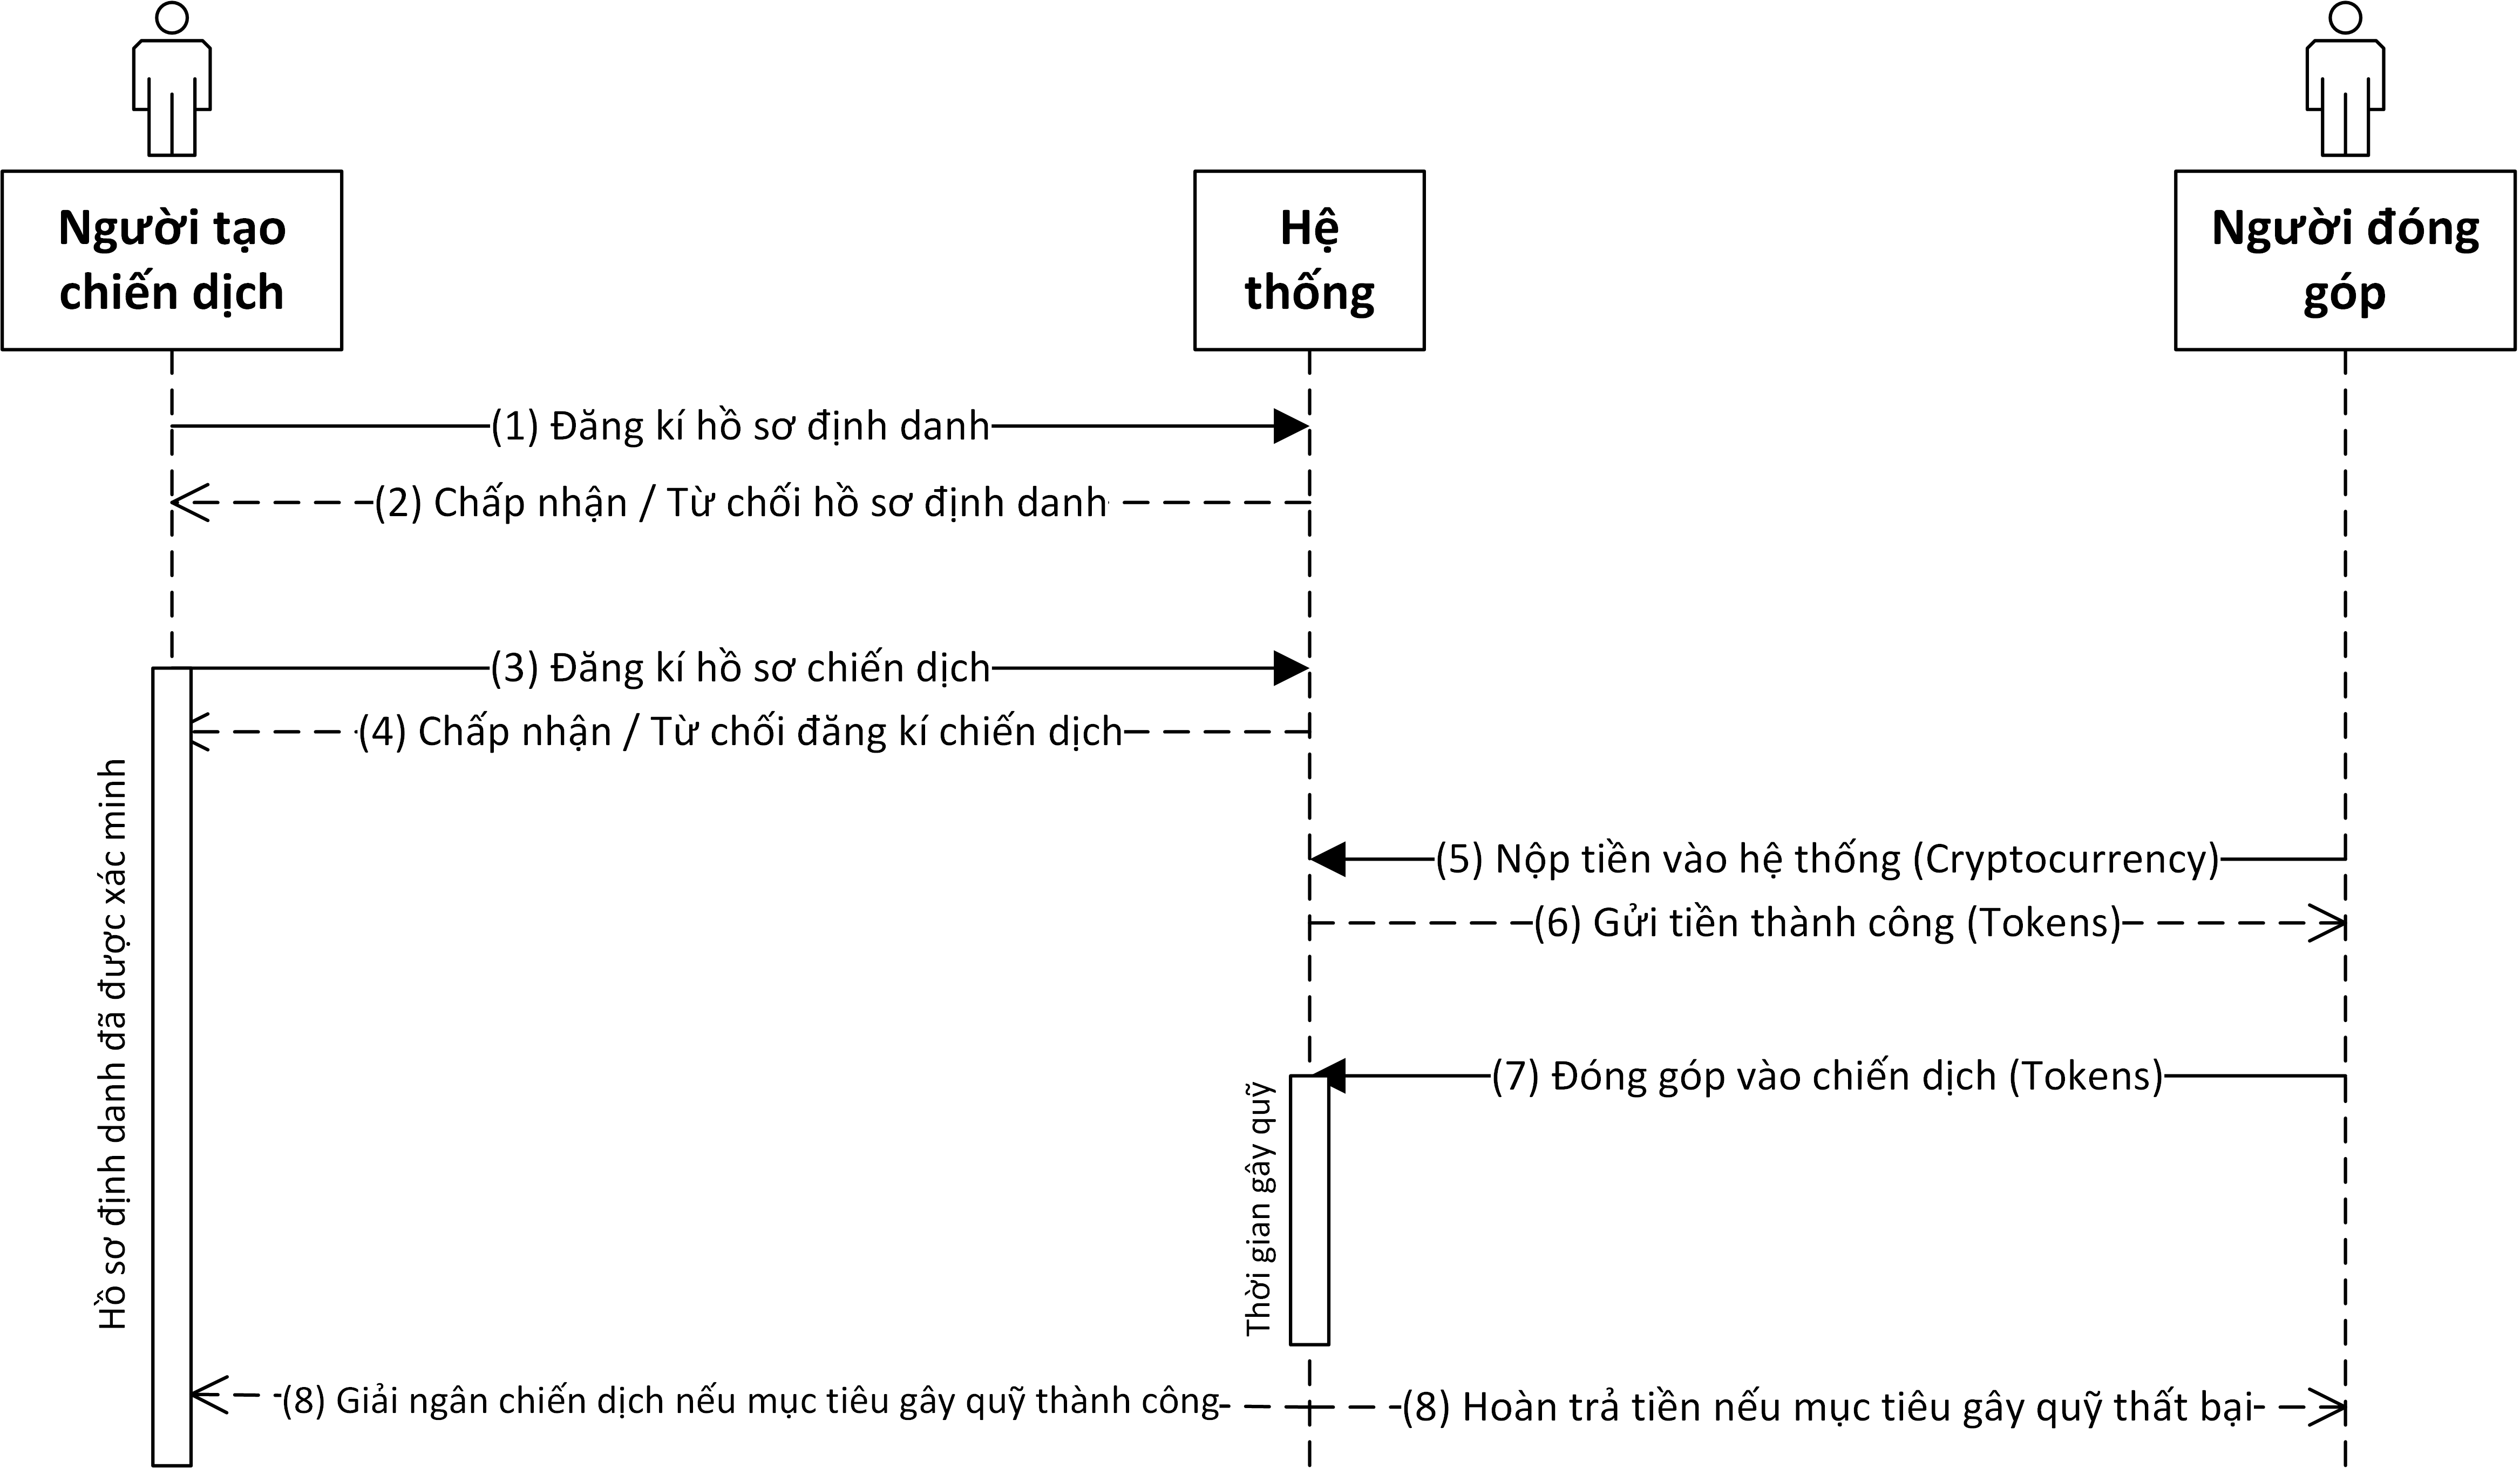
\includegraphics[scale=0.75]{crowdfunding-process}
\caption{Sơ đồ quy trình gây quỹ cộng đồng}
\end{center}
\end{figure}

Quy trình này được diễn giải như sau:

\begin{enumerate}[label=(\arabic*)]
\item Người tạo chiến dịch sẽ tiến hành tạo lập hồ sơ định danh bao gồm thông tin cá nhân cơ bản và thông tin chứng minh định danh.
\item Hệ thống (nhân viên xác minh) tiến hành xác minh hồ sơ định danh và chấp nhận hay từ chối hồ sơ. Nếu hồ sơ định danh được chấp nhận thì hồ sơ đó được phép gọi lệnh tạo chiến dịch, ngược lại thì không.
\item Người tạo chiến dịch tiếp tục tạo lập hồ sơ chiến dịch gây quỹ nếu hồ sơ định danh được chấp nhận.
\item Hệ thống (nhân viên xác minh) tiến hành xác minh hồ sơ chiến dịch và chấp nhận hay từ chối hồ sơ. Hồ sơ được chấp nhận sẽ được công khai lên hệ thống và cho phép người đóng góp ủng hộ tiền. Ngược lại thì không.
\item Người đóng góp muốn ủng hộ tiền cho một chiến dịch thì cần sử dụng \gls{cryptocurrency} (\glsdesc{cryptocurrency}) gửi vào hệ thống (lúc này là hợp đồng thông minh) để sử dụng các chức năng trong hệ thống.
\item Sau khi người đóng góp gửi tiền vào hệ thống, hệ thống sẽ lưu số tiền người gửi vào dưới dạng một giá trị được gọi là token. Người đóng góp sử dụng token này trong các giao dịch nội bộ của hệ thống. Token này có thể được đổi ngược lại sang đồng \gls{cryptocurrency} với giá tương ứng
\item Người đóng góp ủng hộ tiền cho một chiến dịch (chiến dịch đã được xác minh) bằng một lượng token mà người đóng góp mong muốn và đang có.
\item Mỗi chiến dịch sẽ có một khoảng thời gian để kêu gọi đóng góp, và một mục tiêu là số lượng token cần đạt được. Khi hết thời gian kêu gọi đóng góp, nếu chiến dịch hoàn thành mục tiêu thì sẽ tiến hành cho người tạo chiến dịch giải ngân. Ngược lại, lượng token đã đóng góp sẽ được hoàn lại cho người đóng góp.
\end{enumerate}
\section{Kiến trúc hệ thống}
Kiến trúc hệ thống được thể hiện ở hình \ref{fig:system-architecture}.

\begin{figure}[ht!]
\begin{center}
\label{fig:system-architecture}
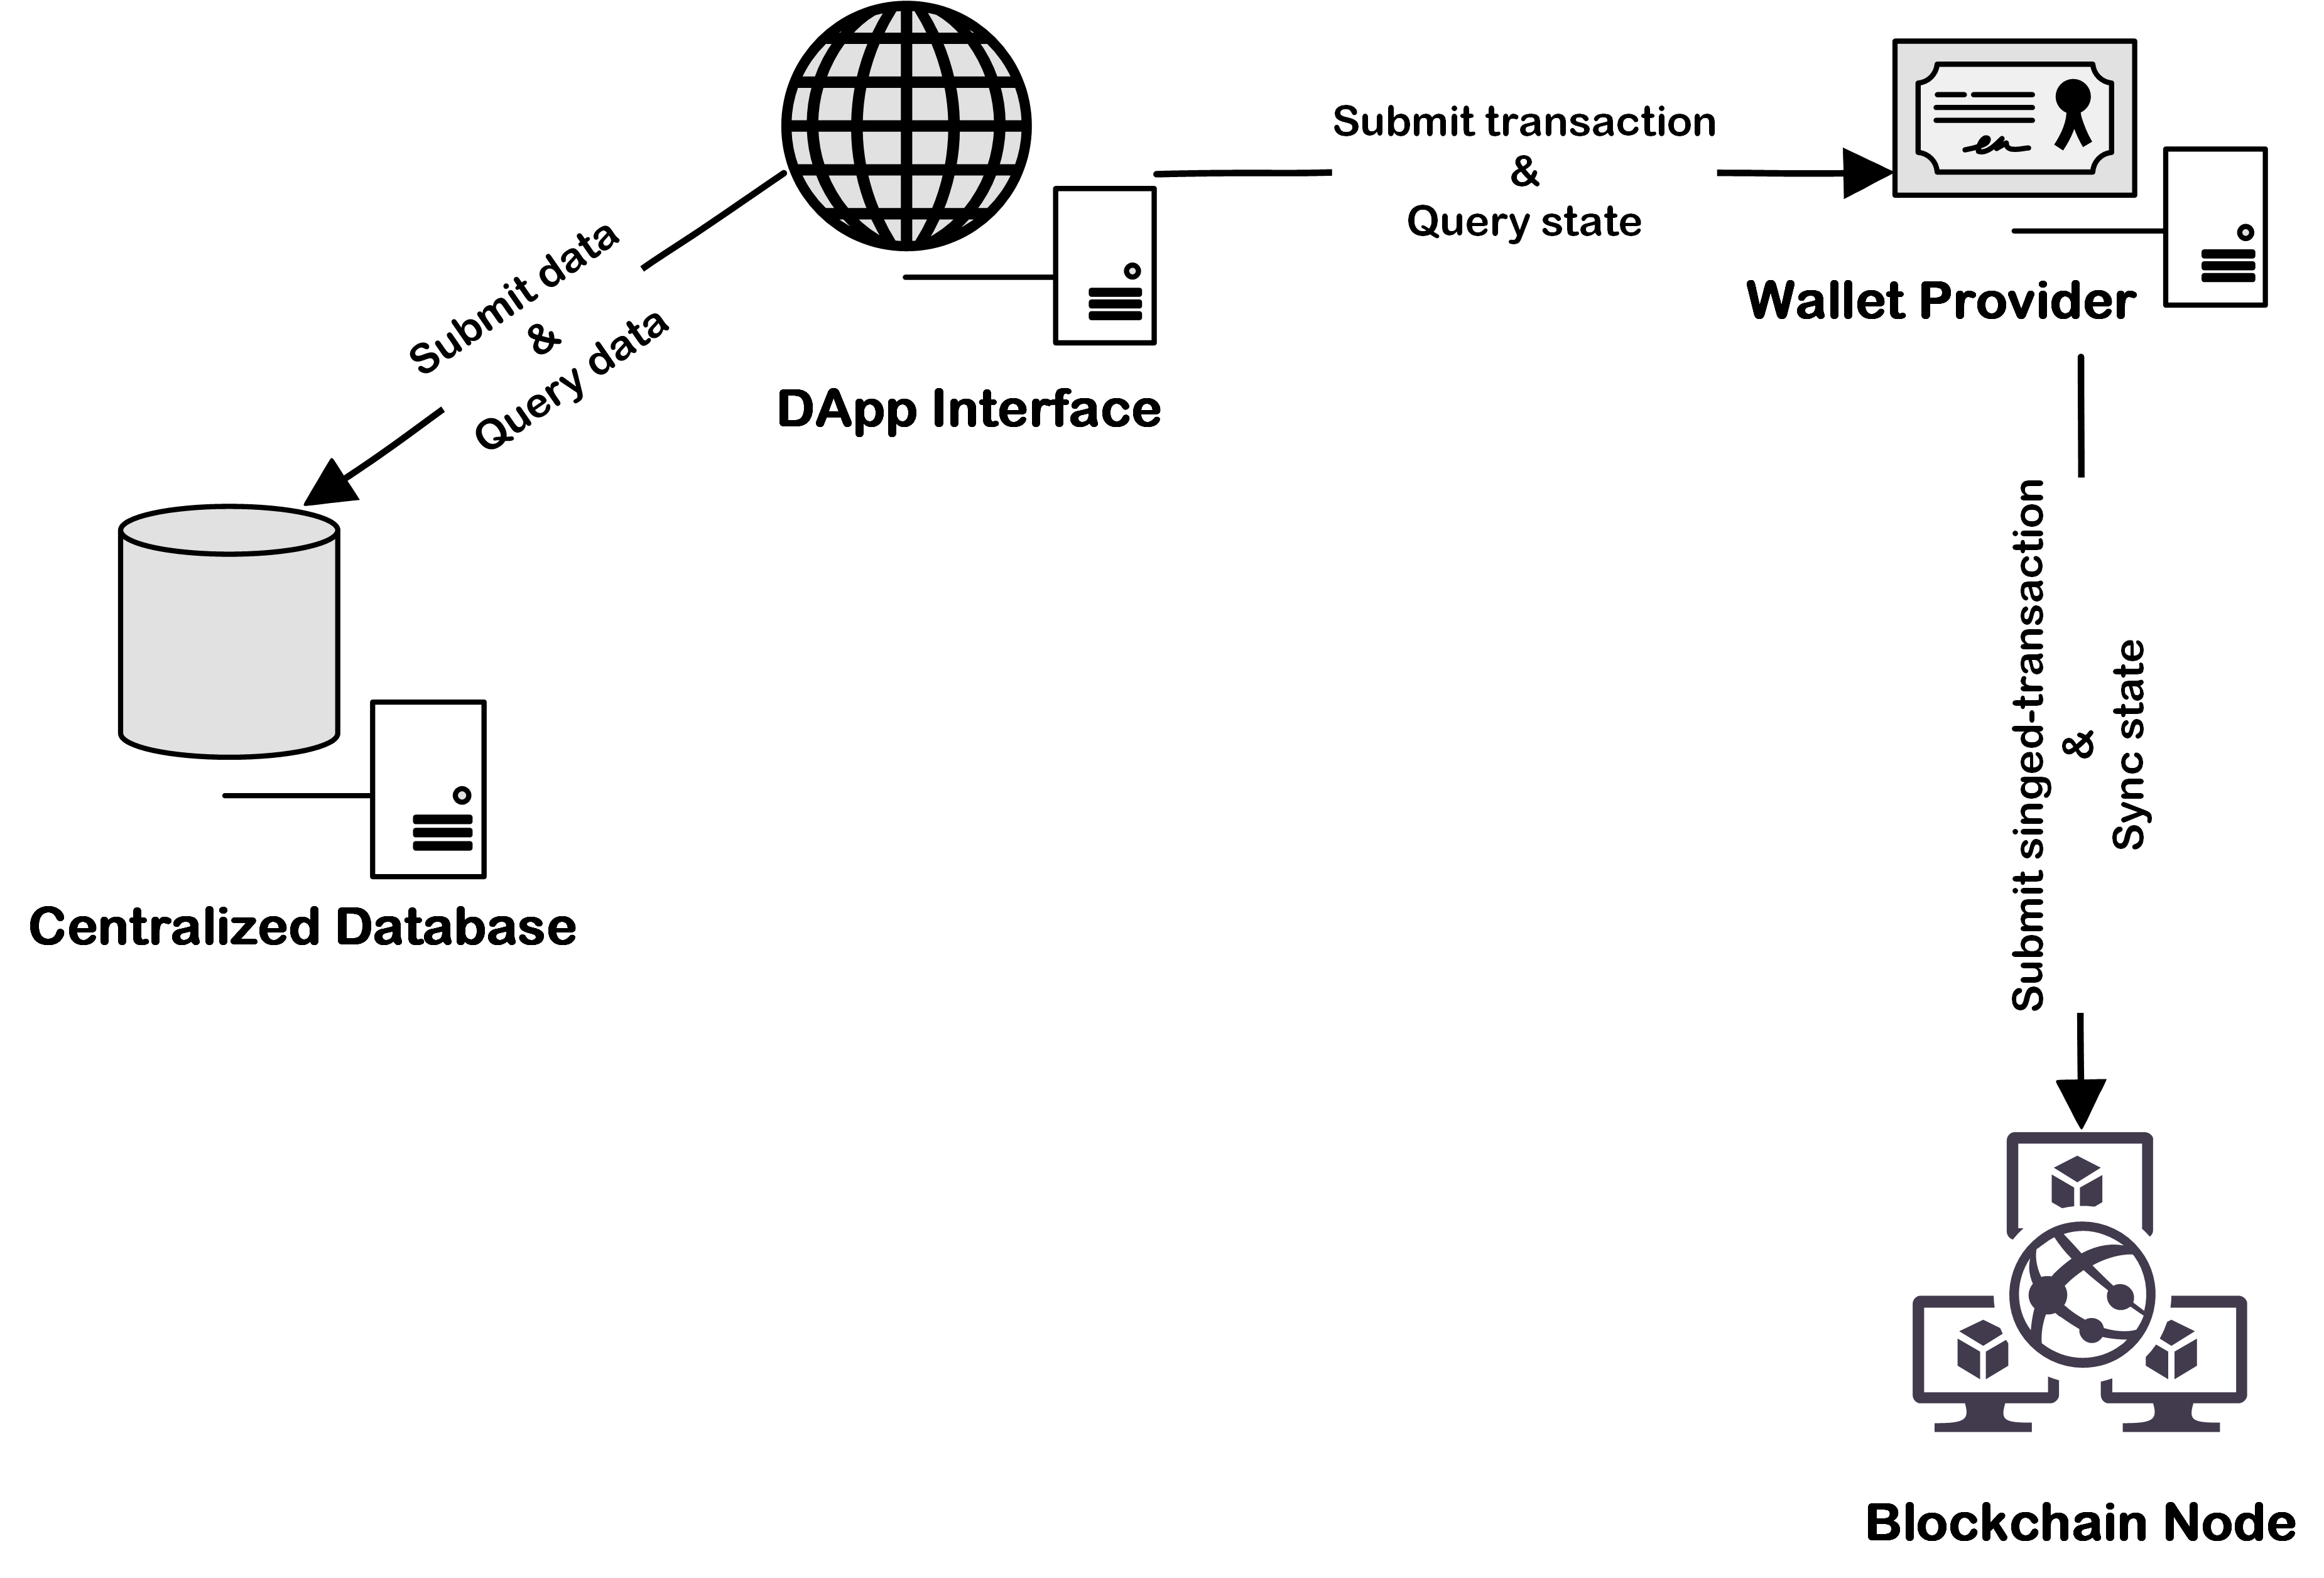
\includegraphics[scale=0.9]{system-architecture}
\caption{Sơ đồ kiến trúc hệ thống}
\end{center}
\end{figure}

Các thành phần và vai trò của từng thành phần trong hệ thống mà nhóm tác giả đề xuất như sau:

\begin{itemize}
\item \textbf{DApp Interface} - là một giao diện ứng dụng phi tập trung, nơi người dùng sẽ tương tác trực tiếp. \textit{DApp Interface} sẽ tạo ra các \gls{transaction} để gọi các hàm có trong hợp đồng thông minh và chuyển các \gls{transaction} này tới Wallet Provider thực hiện công đoạn tiếp theo. Và đây cũng là nơi tương tác với cơ sở dữ liệu tập trung trong mô hình. Thực chất \textit{DApp Interface} chỉ là một giao diện front-end tĩnh chạy ở phía người dùng.
\item \textbf{Wallet Provider} - là ứng dụng phi tập trung có nhiệm vụ xác nhận và kí transaction (\textit{sign transaction}) do \textit{DApp Interfac}e gửi tới trong mô hình, sau đó thực hiện gửi các \gls{transaction} đã được kí (\textit{signed-transaction}) đến mạng lưới \gls{blockchain}. Wallet cũng làm nhiệm vụ lưu trữ thông tin về khóa bí mật của người dùng.
\item \textbf{Blokchain Node} - là một nút trong mạng \gls{blockchain} mà \textit{Wallet Provider} tương tác để lưu trữ các dữ liệu phi tập trung, các dữ liệu phi tập trung trong trường hợp này là các mã hợp đồng thông tin và các giá trị trong hợp đồng.
\item \textbf{Centralized Database} - là một cơ sở dữ liệu tập trung, được dùng để lưu trữ một số thông tin như mô tả chiến dịch.
\end{itemize}

\section{Các chức năng}
\subsection{Tổng quan các chức năng}
Tổng quan các chức năng trong hệ thống được thể hiện ở hình \ref{fig:usecase-diagram}.

\begin{figure}[ht!]
\begin{center}
\label{fig:usecase-diagram}
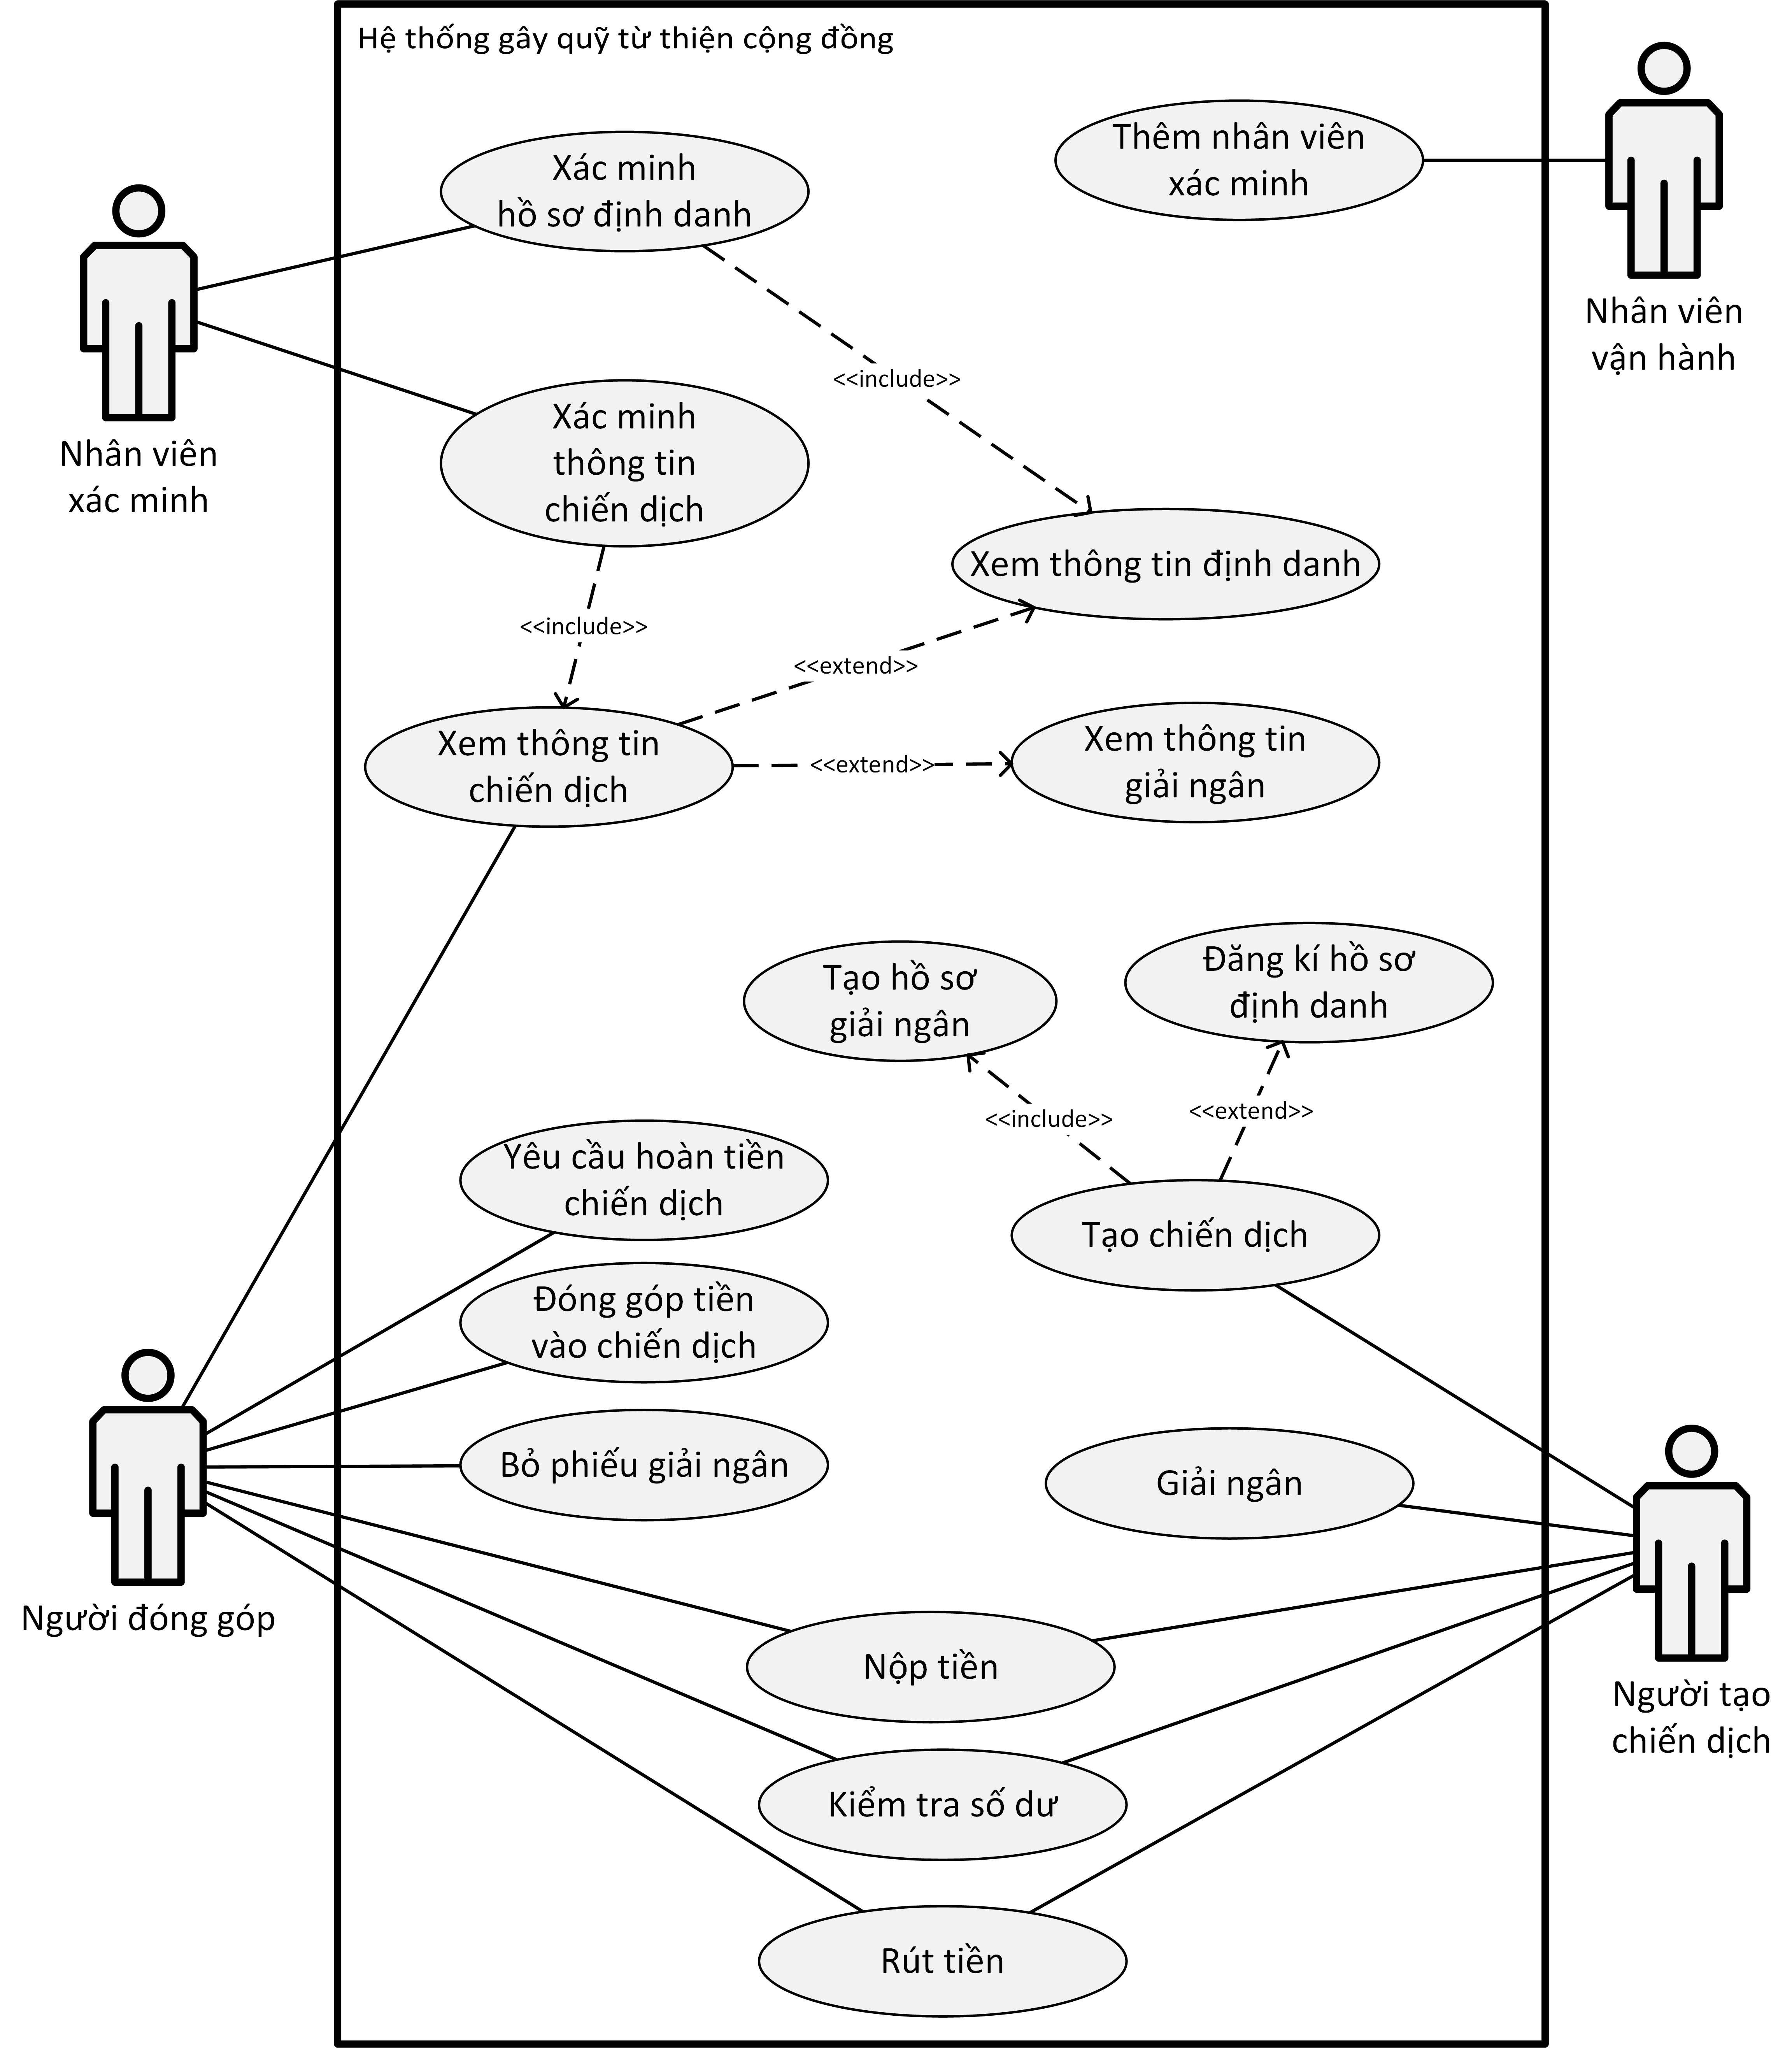
\includegraphics[scale=0.6]{usecase-vi}
\caption{Sơ đồ tổng quan các chức năng trong hệ thống}
\end{center}
\end{figure}

Với sơ đồ được thể hiện có các đối tượng sau:

\begin{itemize}
\item \textbf{Người tạo chiến dịch} - là người tạo chiến dịch gây quỹ.
\item \textbf{Người đóng góp} - là người đóng góp, ủng hộ tiền cho chiến dịch gây quỹ.
\item \textbf{Nhân viên xác minh} - là người xác minh cho hồ sơ định danh và hồ sơ gây quỹ, là nhân viên trong hệ thống hoặc tình nguyện viên của hệ thống.
\item \textbf{Nhân viên vận hành} - là người vận hành hệ thống hay người triển khai các hợp đồng thông minh.
\end{itemize}

Nhóm tác giả cũng thực hiện phân rã các chức năng và được sơ đồ như ở hình \ref{fig:function-tree}.

\begin{figure}[ht!]
\begin{center}
\label{fig:function-tree}
\fbox{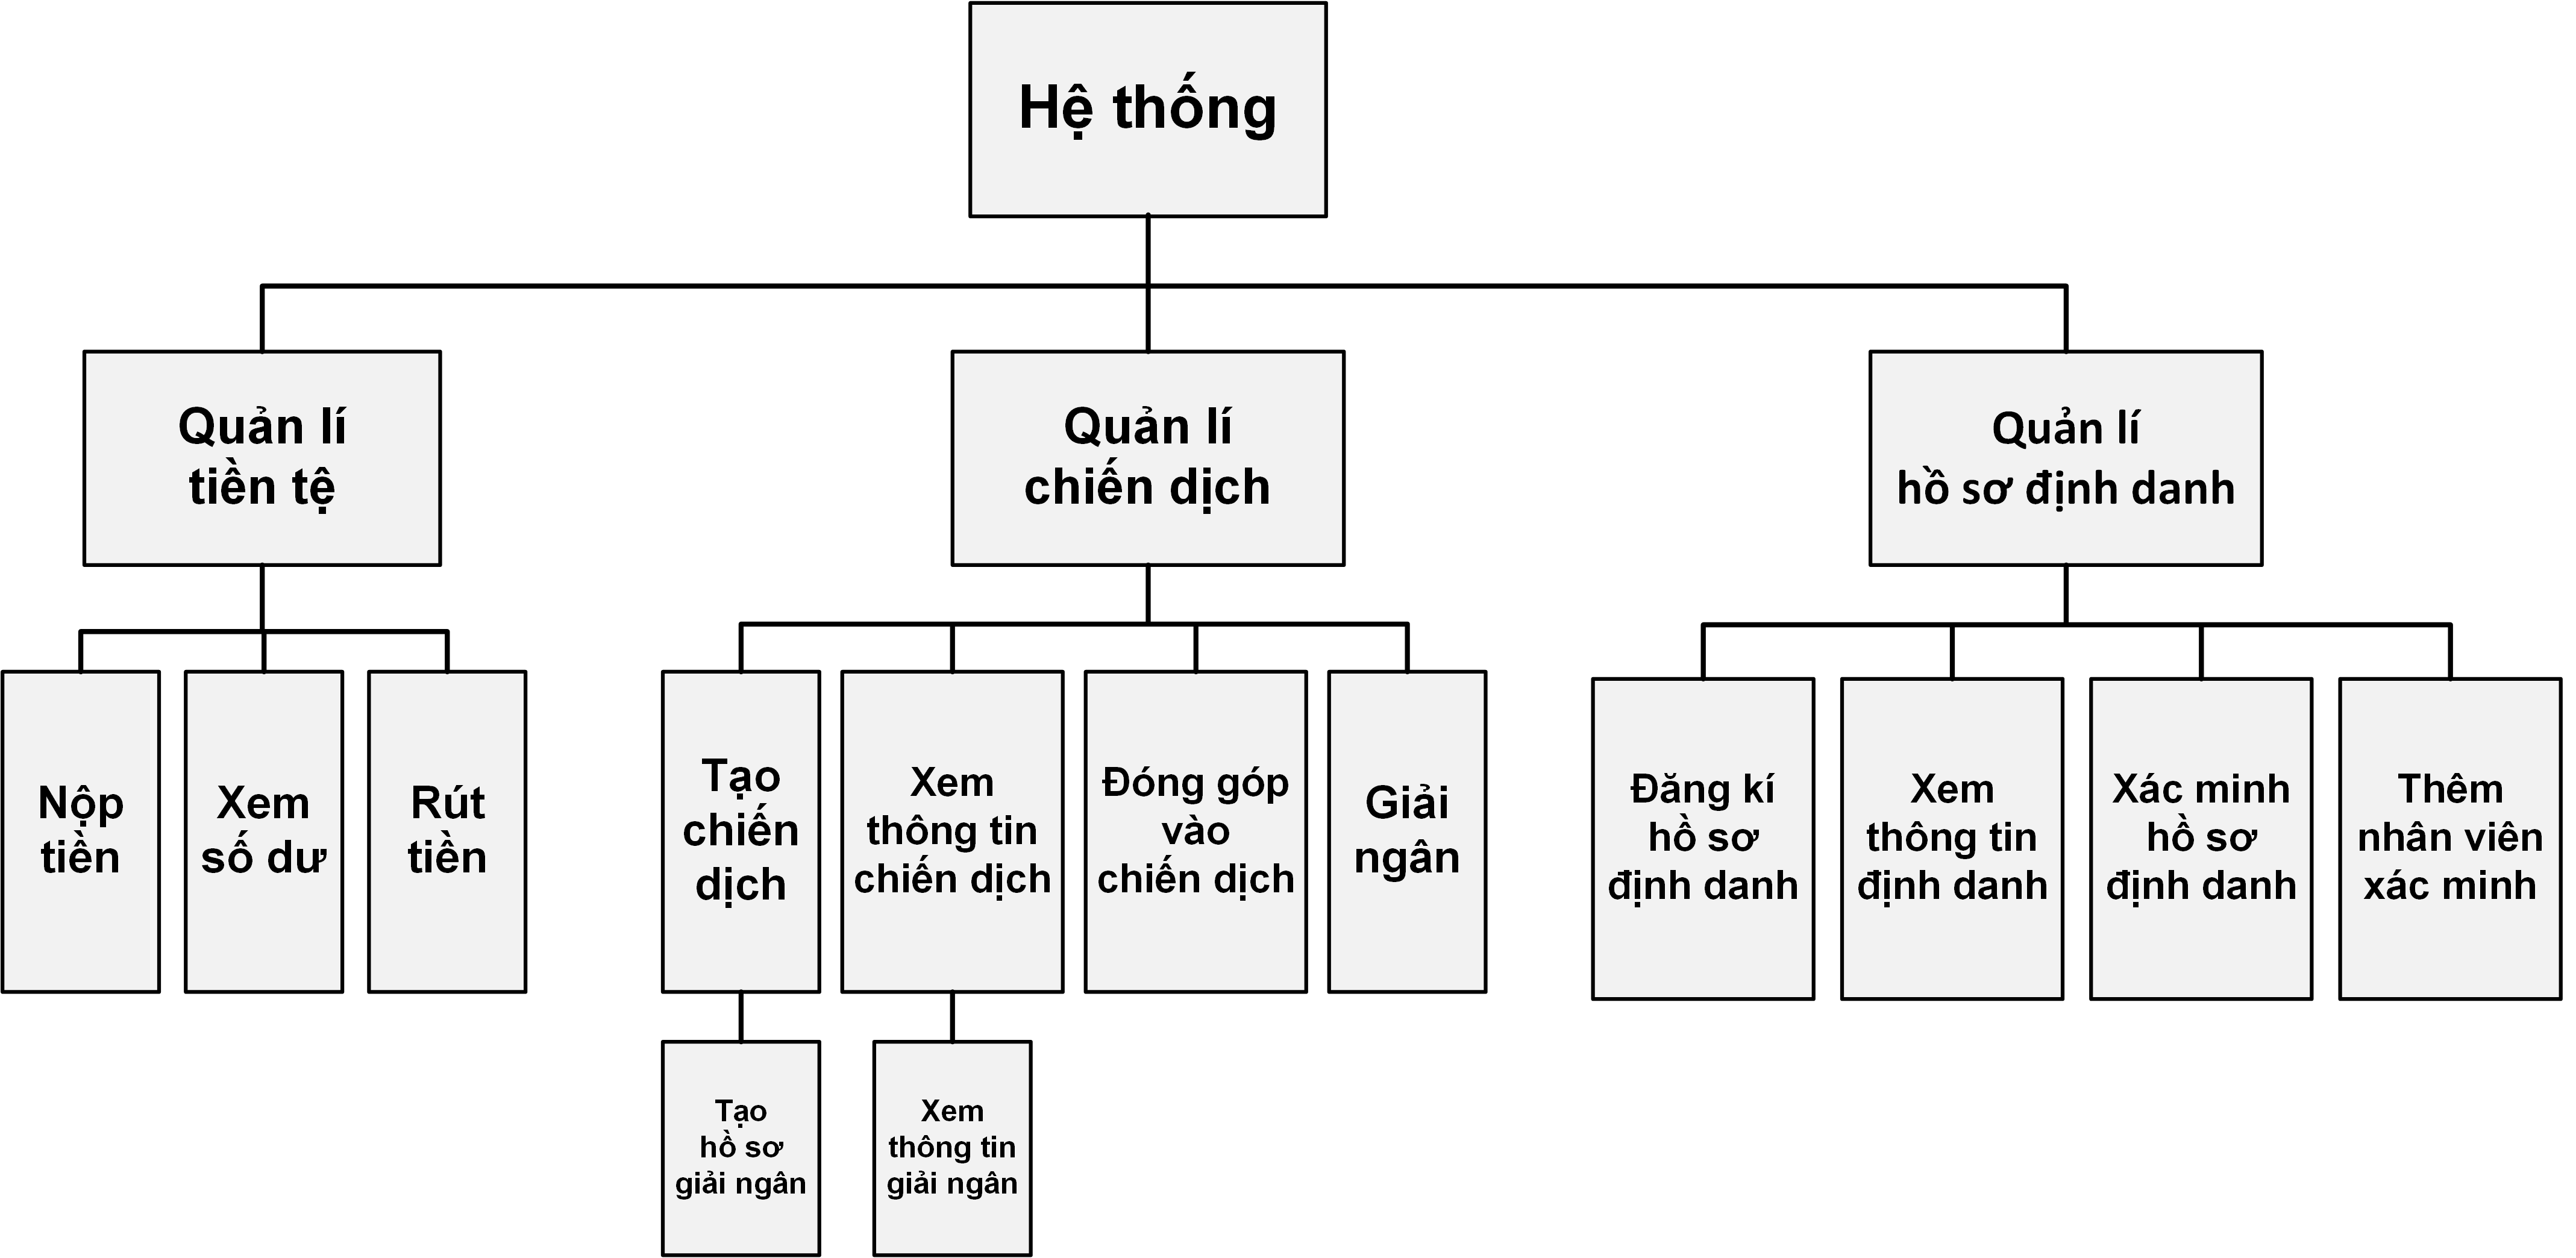
\includegraphics[scale=0.7]{function-tree}}
\caption{Sơ đồ phân rã các chức năng trong hệ thống}
\end{center}
\end{figure}

Tiếp theo là sơ đồ ở hình \ref{fig:user-data-flow} thể hiện tổng quan về các đối tượng và luồng tương tác dữ liệu giữa các đối tượng. Đối tượng \textbf{``Hệ thống''} trong sơ đồ được nhóm tác giả đặc tả một cách khái quát cho toàn thể hệ thống.

\begin{figure}[ht!]
\begin{center}
\label{fig:user-data-flow}
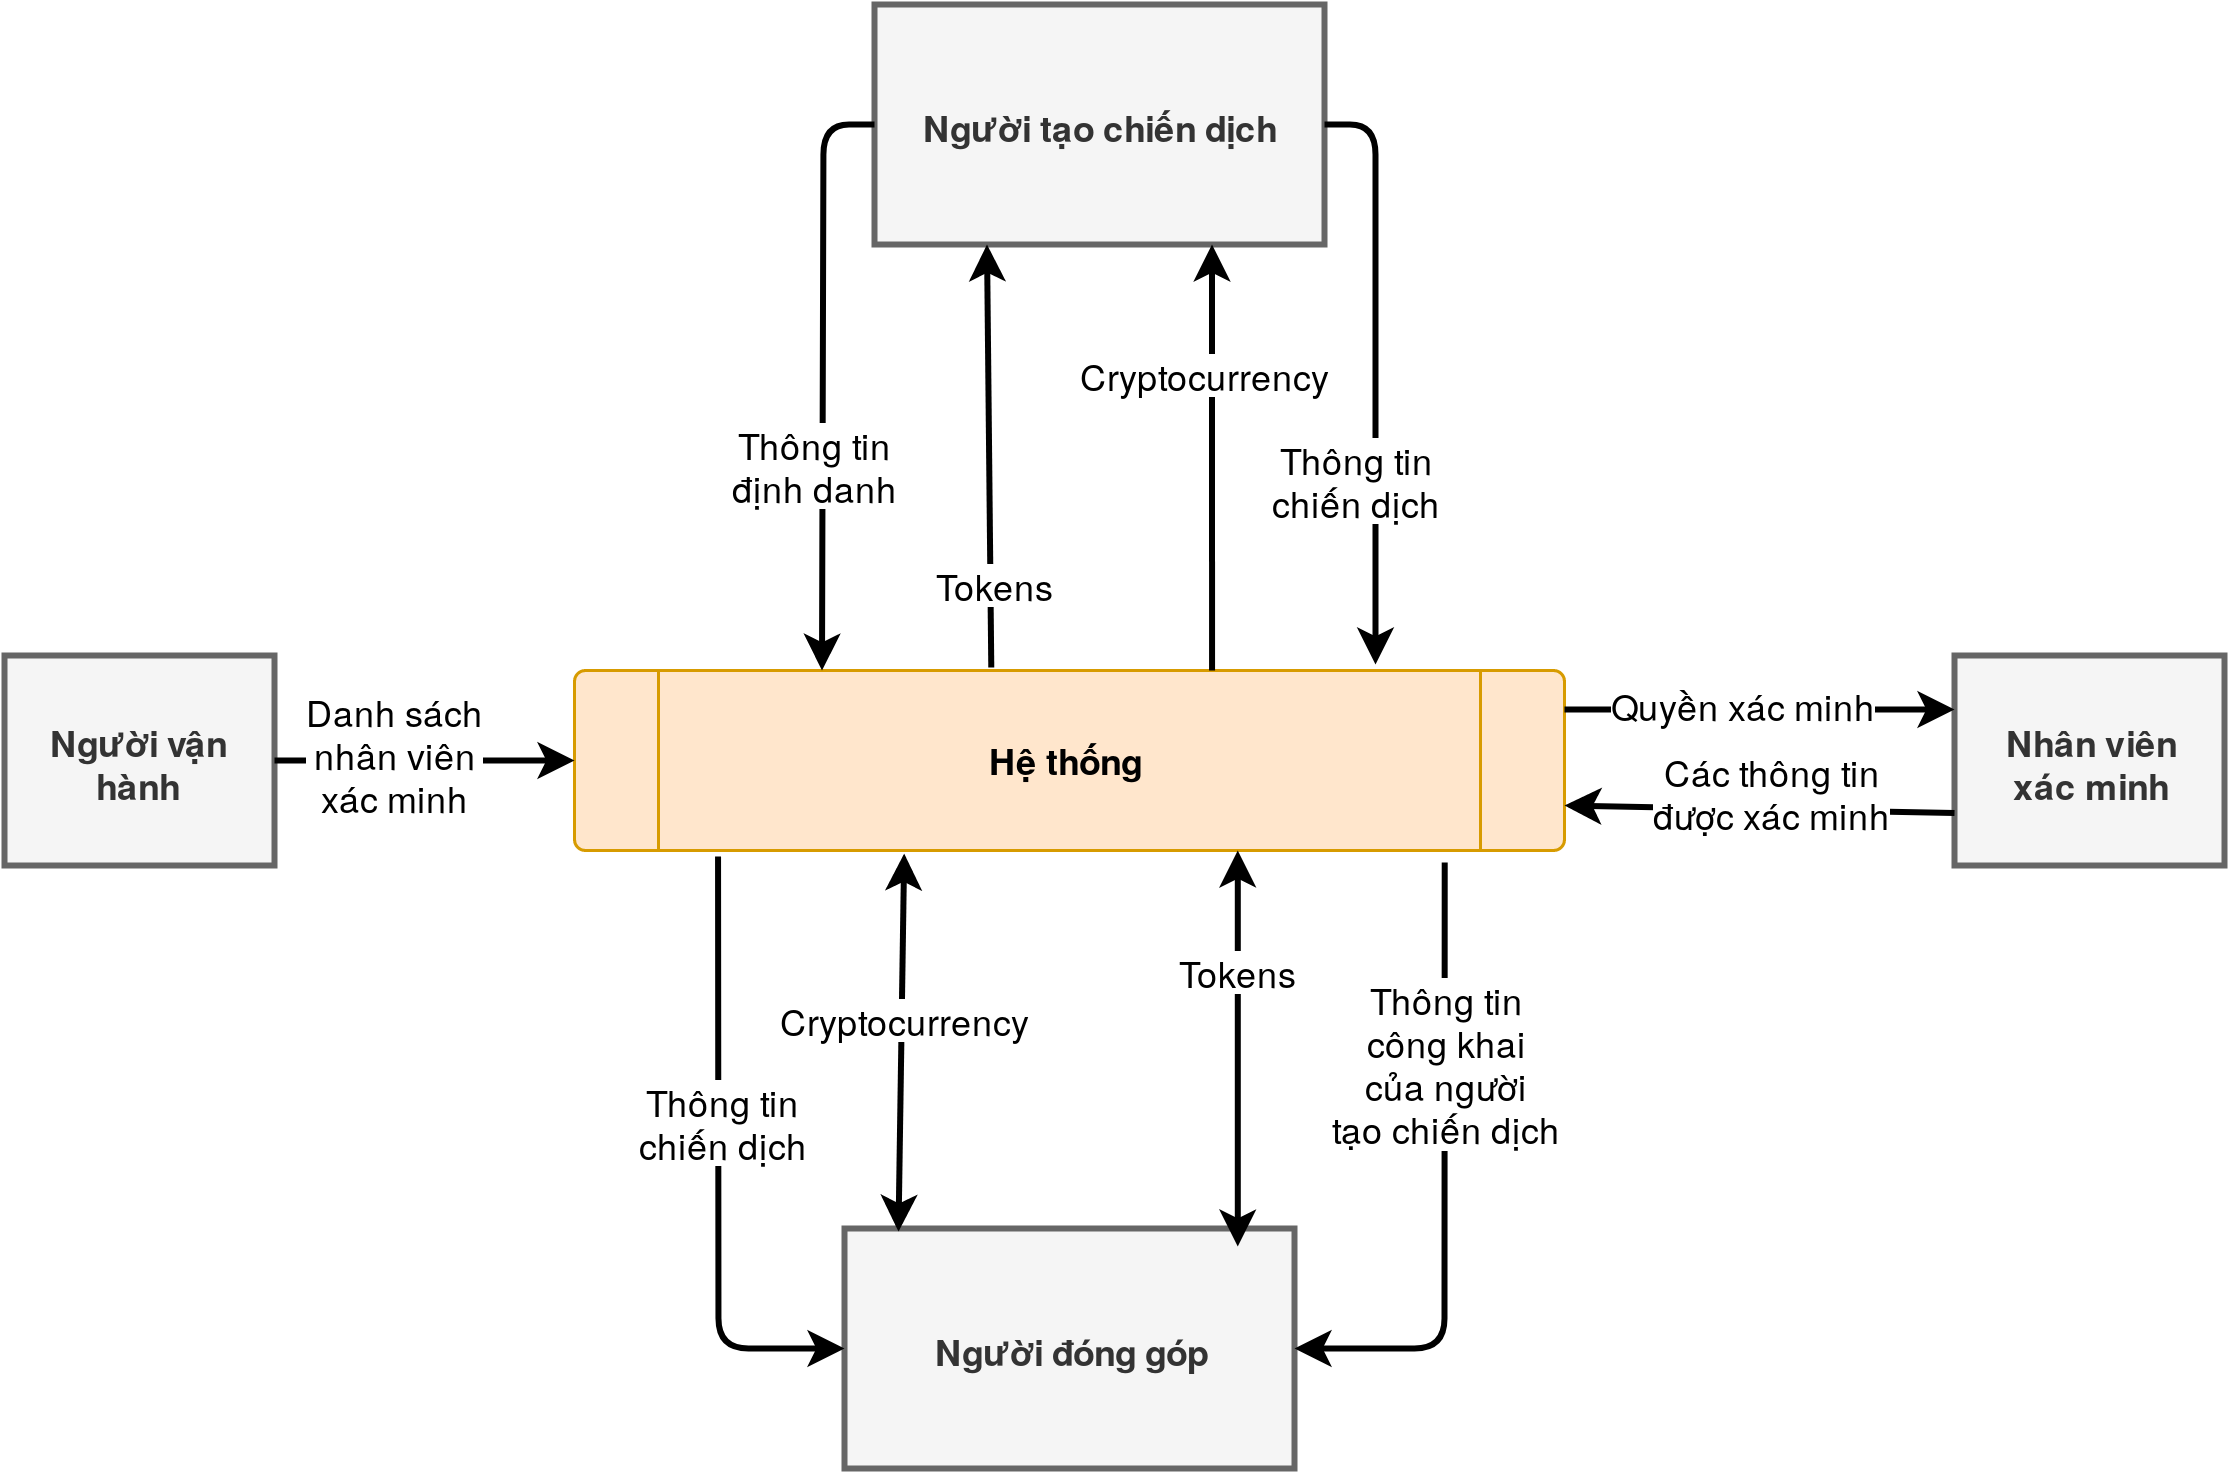
\includegraphics[scale=0.18]{user-data-flow}
\caption{Sơ đồ tổng quan các đối tượng và luồng tương tác dữ liệu}
\end{center}
\end{figure}

\subsection{Chức năng nộp tiền và rút tiền}
\subsubsection{Mục tiêu}
Trong mô hình hệ thống mà nhóm tác giả đề xuất, người đóng góp sẽ ủng hộ cho chiến dịch gây quỹ từ thiện thông qua tiền mã hóa. Trong thời gian kêu gọi quỹ, người tạo chiến dịch chưa nhận được bất kì lượng tiền nào, chỉ khi nào chiến dịch kêu gọi đạt được mục tiêu thì người tạo chiến dịch mới thực sự nhận được tiền. Để đạt được yêu cầu như vậy thì trong thời gian kêu gọi quỹ, người đóng góp chỉ thật sự ủng hộ trên danh nghĩa là đồng ý đóng góp khoản tiền nào đó chứ không chuyển trực tiếp cho người tạo chiến dịch. Việc ủng hộ trên danh nghĩa này phải được đảm bảo rằng sau khi chiến dịch kết thúc, người tạo chiến dịch sẽ nhận được đúng số tiền ủng hộ. Do đó, trong trường hợp này sẽ cần xuất hiện một bên thứ ba, làm nhiệm vụ giữ tiền và trao đổi tiền giữa hai bên. Như đã được giới thiệu từ trước, hợp đồng thông minh đảm bảo việc thực thi các luồng xử lí một cách tự động mà không có sự can thiệp từ yếu tố con người làm sai lệch kết quả. Nên sử dụng hợp đồng để lưu giữ tiền cam kết giữa hai bên và xử lí các điều kiện để giải ngân cho chiến dịch là hợp lí. Vì vậy cần có chức năng gửi tiền và rút tiền từ hợp đồng thông minh với mục tiêu sau:

\begin{itemize}
\item Người đóng góp sẽ gửi tiền mã hóa vào hợp đồng minh và nhận lại một giá trị lưu trữ cho số tiền gửi vào. Giá trị này được gọi là \textbf{token}.
\item Token được sử dụng cho các hoạt động trong hệ thống, bao gồm đóng góp vào chiến dịch gây quỹ.
\item Token cũng được quy đổi ngược lại đồng tiền mã hóa theo một tỉ lệ tương ứng nhất định. Đây là chức năng rút tiền trong hệ thống.
\item Tỉ lệ quy đổi sẽ do người vận hành hệ thống quyết định.
\item Giá trị token của người dùng đã gửi vào luôn không thay đổi trong suốt quá trình tham gia hệ thống. Ngoại trừ hoạt động rút tiền và đóng góp cho chiến dịch.
\end{itemize}

\subsubsection{Cách thức hoạt động}
Sơ đồ hoạt động chức năng nộp tiền được thể hiện ở hình \ref{fig:deposit-activity}.

\begin{figure}[ht!]
\begin{center}
\label{fig:deposit-activity}
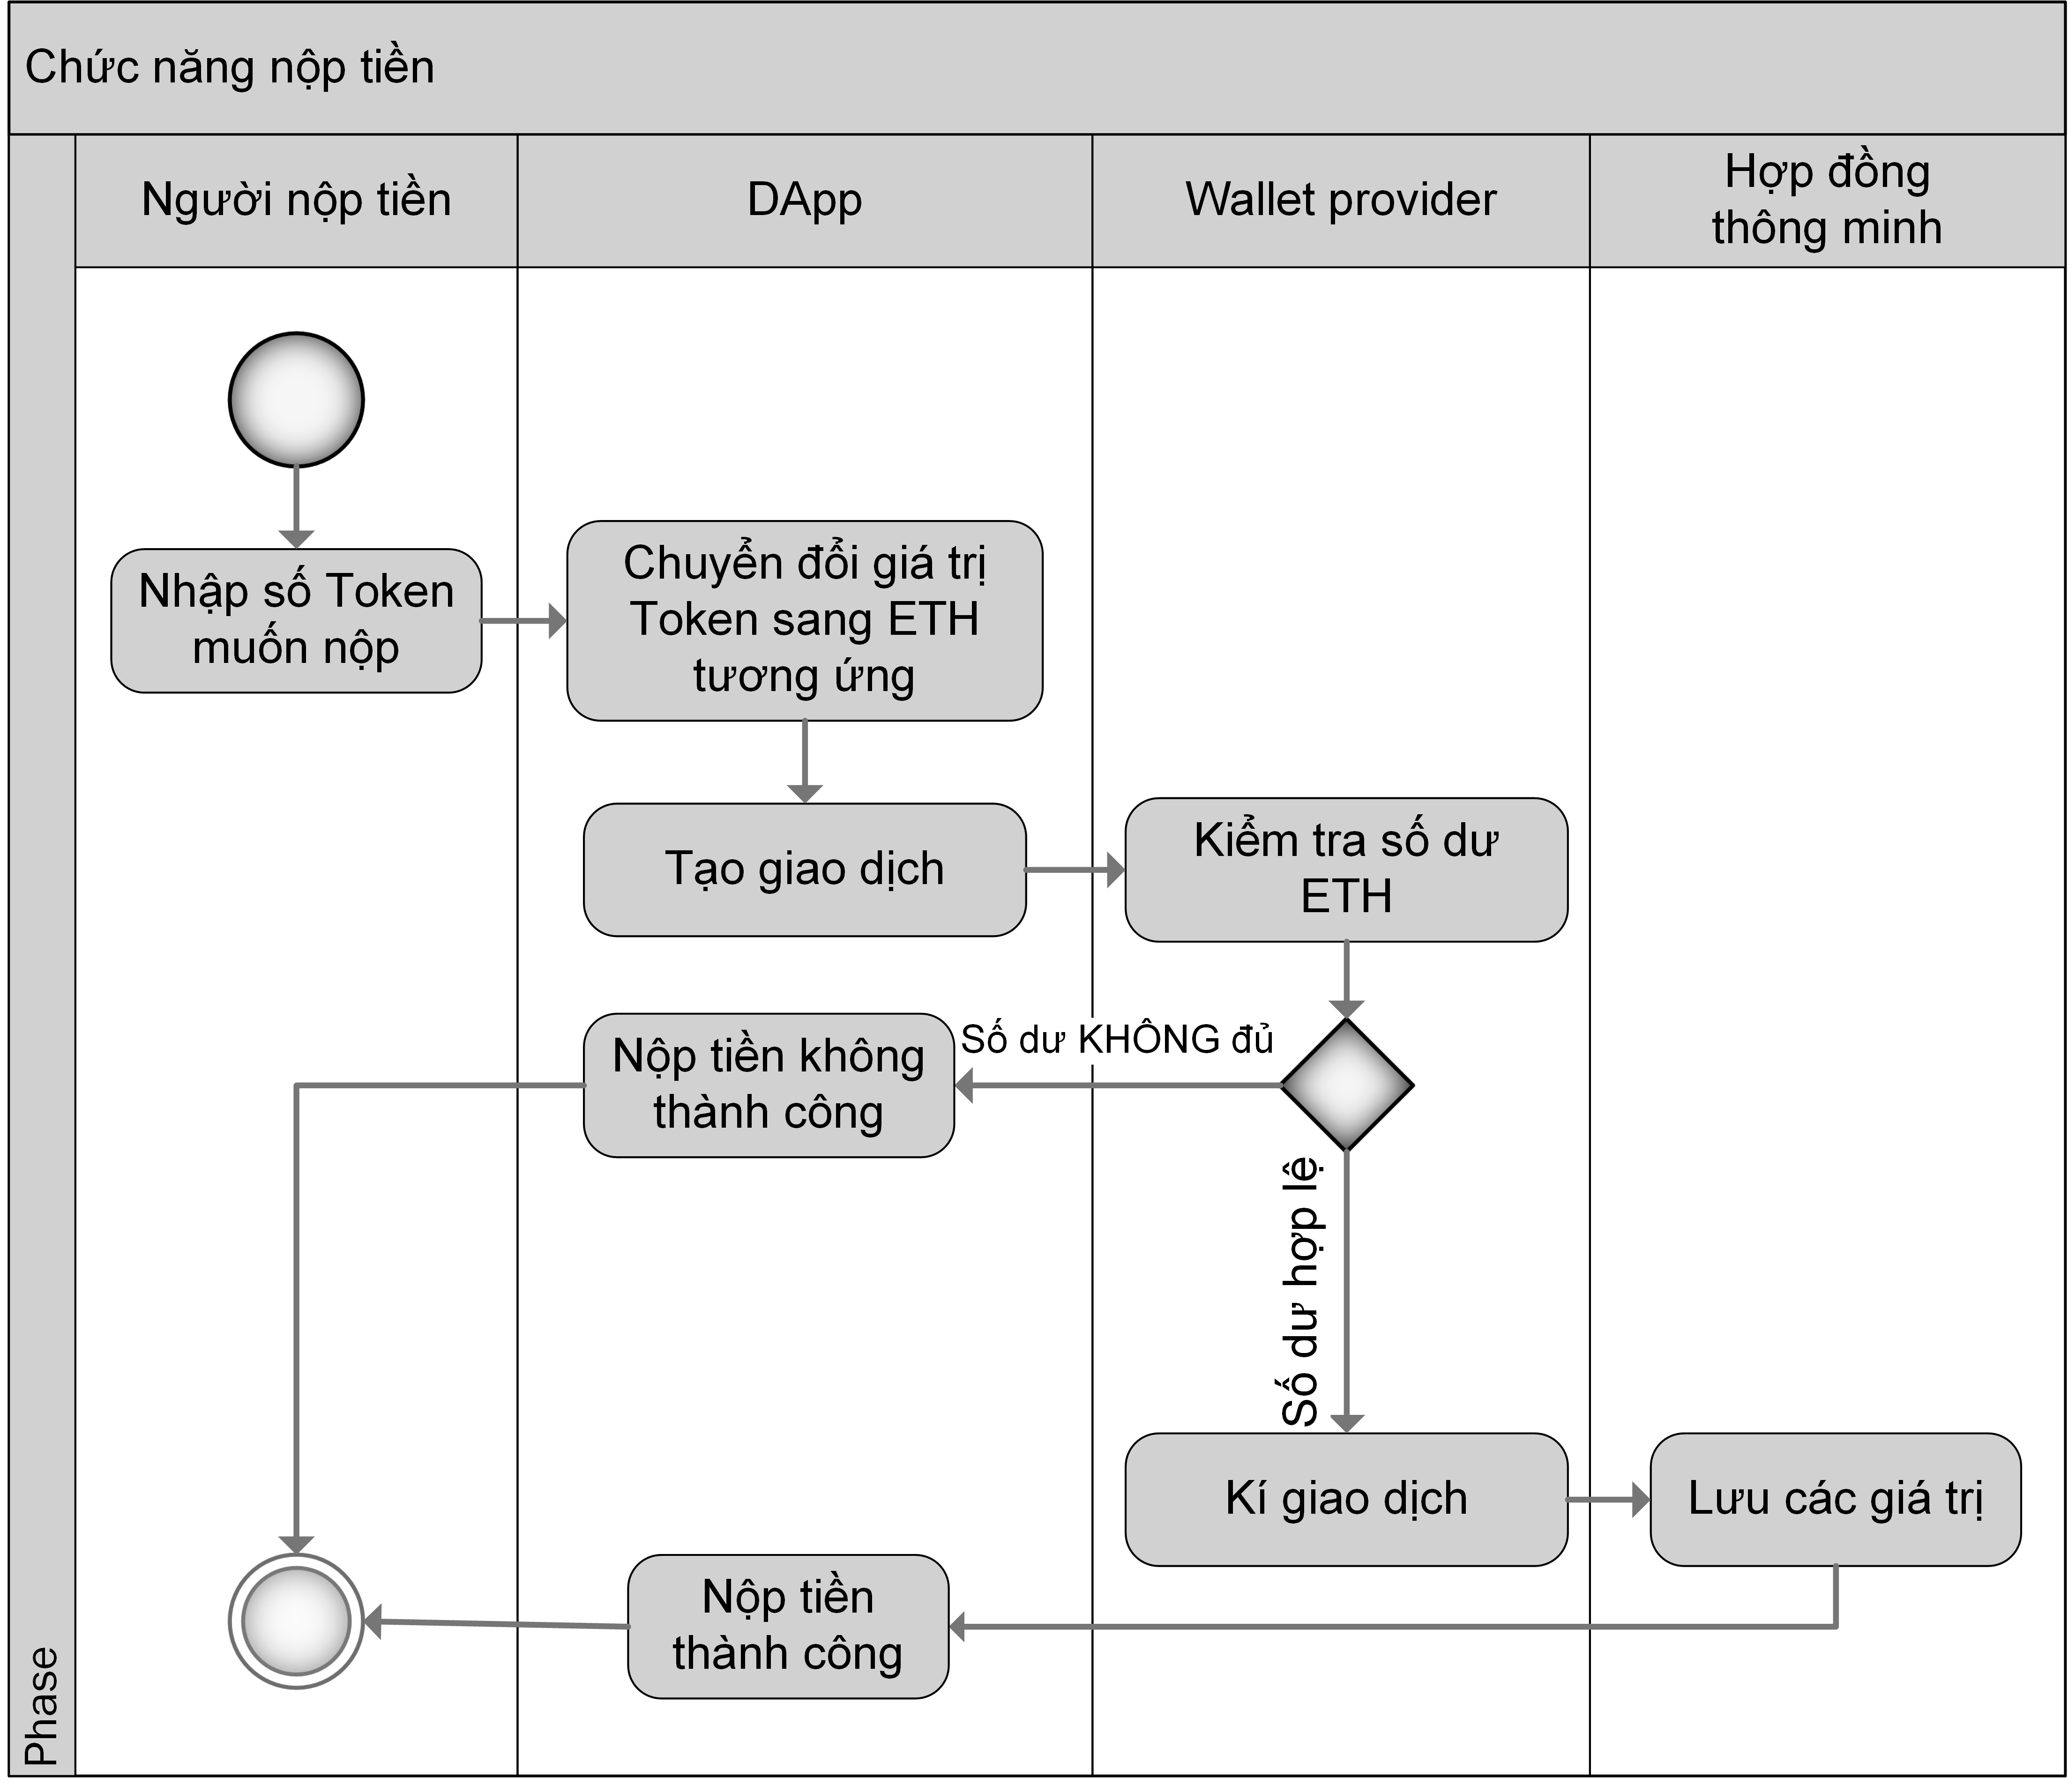
\includegraphics[scale=0.8]{deposit-activity}
\caption{Sơ đồ hoạt động chức năng nộp tiền}
\end{center}
\end{figure}

Tiến trình của hoạt động rút tiền được diễn ra như sau:

\begin{enumerate}[label=(\arabic*)]
\item Người dùng nhập vào lượng token muốn gửi vào hệ thống.
\item Trên giao diện DApp thực hiện tính toán giá trị token và quy đổi sang lượng \gls{eth} tương ứng.
\item DApp tiến hành tạo \gls{transaction} và gửi đến Wallet provider.
\item Wallet provider tiến hành kiểm tra số dư \gls{eth} của người dùng.
\item Nếu số dư đủ để tiến hành giao dịch thì Wallet provider bắt đầu kí transaction và gửi tới một nút trong mạng blockchain. Ngược lại, hiển thị thông báo lỗi cho người dùng trên giao diện DApp.
\item Một nút trong blockchain nhận được transaction từ Wallet provider, lúc này hàm gửi tiền trong hợp đồng thông minh được thực thi. Hợp đồng thông minh tiến hành lưu trữ giá trị token.
\item Hiển thị thông báo gửi tiền thành công và kết thúc tiến trình.
\end{enumerate}

Sơ đồ hoạt động chức năng rút tiền được thể hiện ở hình \ref{fig:withdraw-activity}.

\begin{figure}[ht!]
\begin{center}
\label{fig:withdraw-activity}
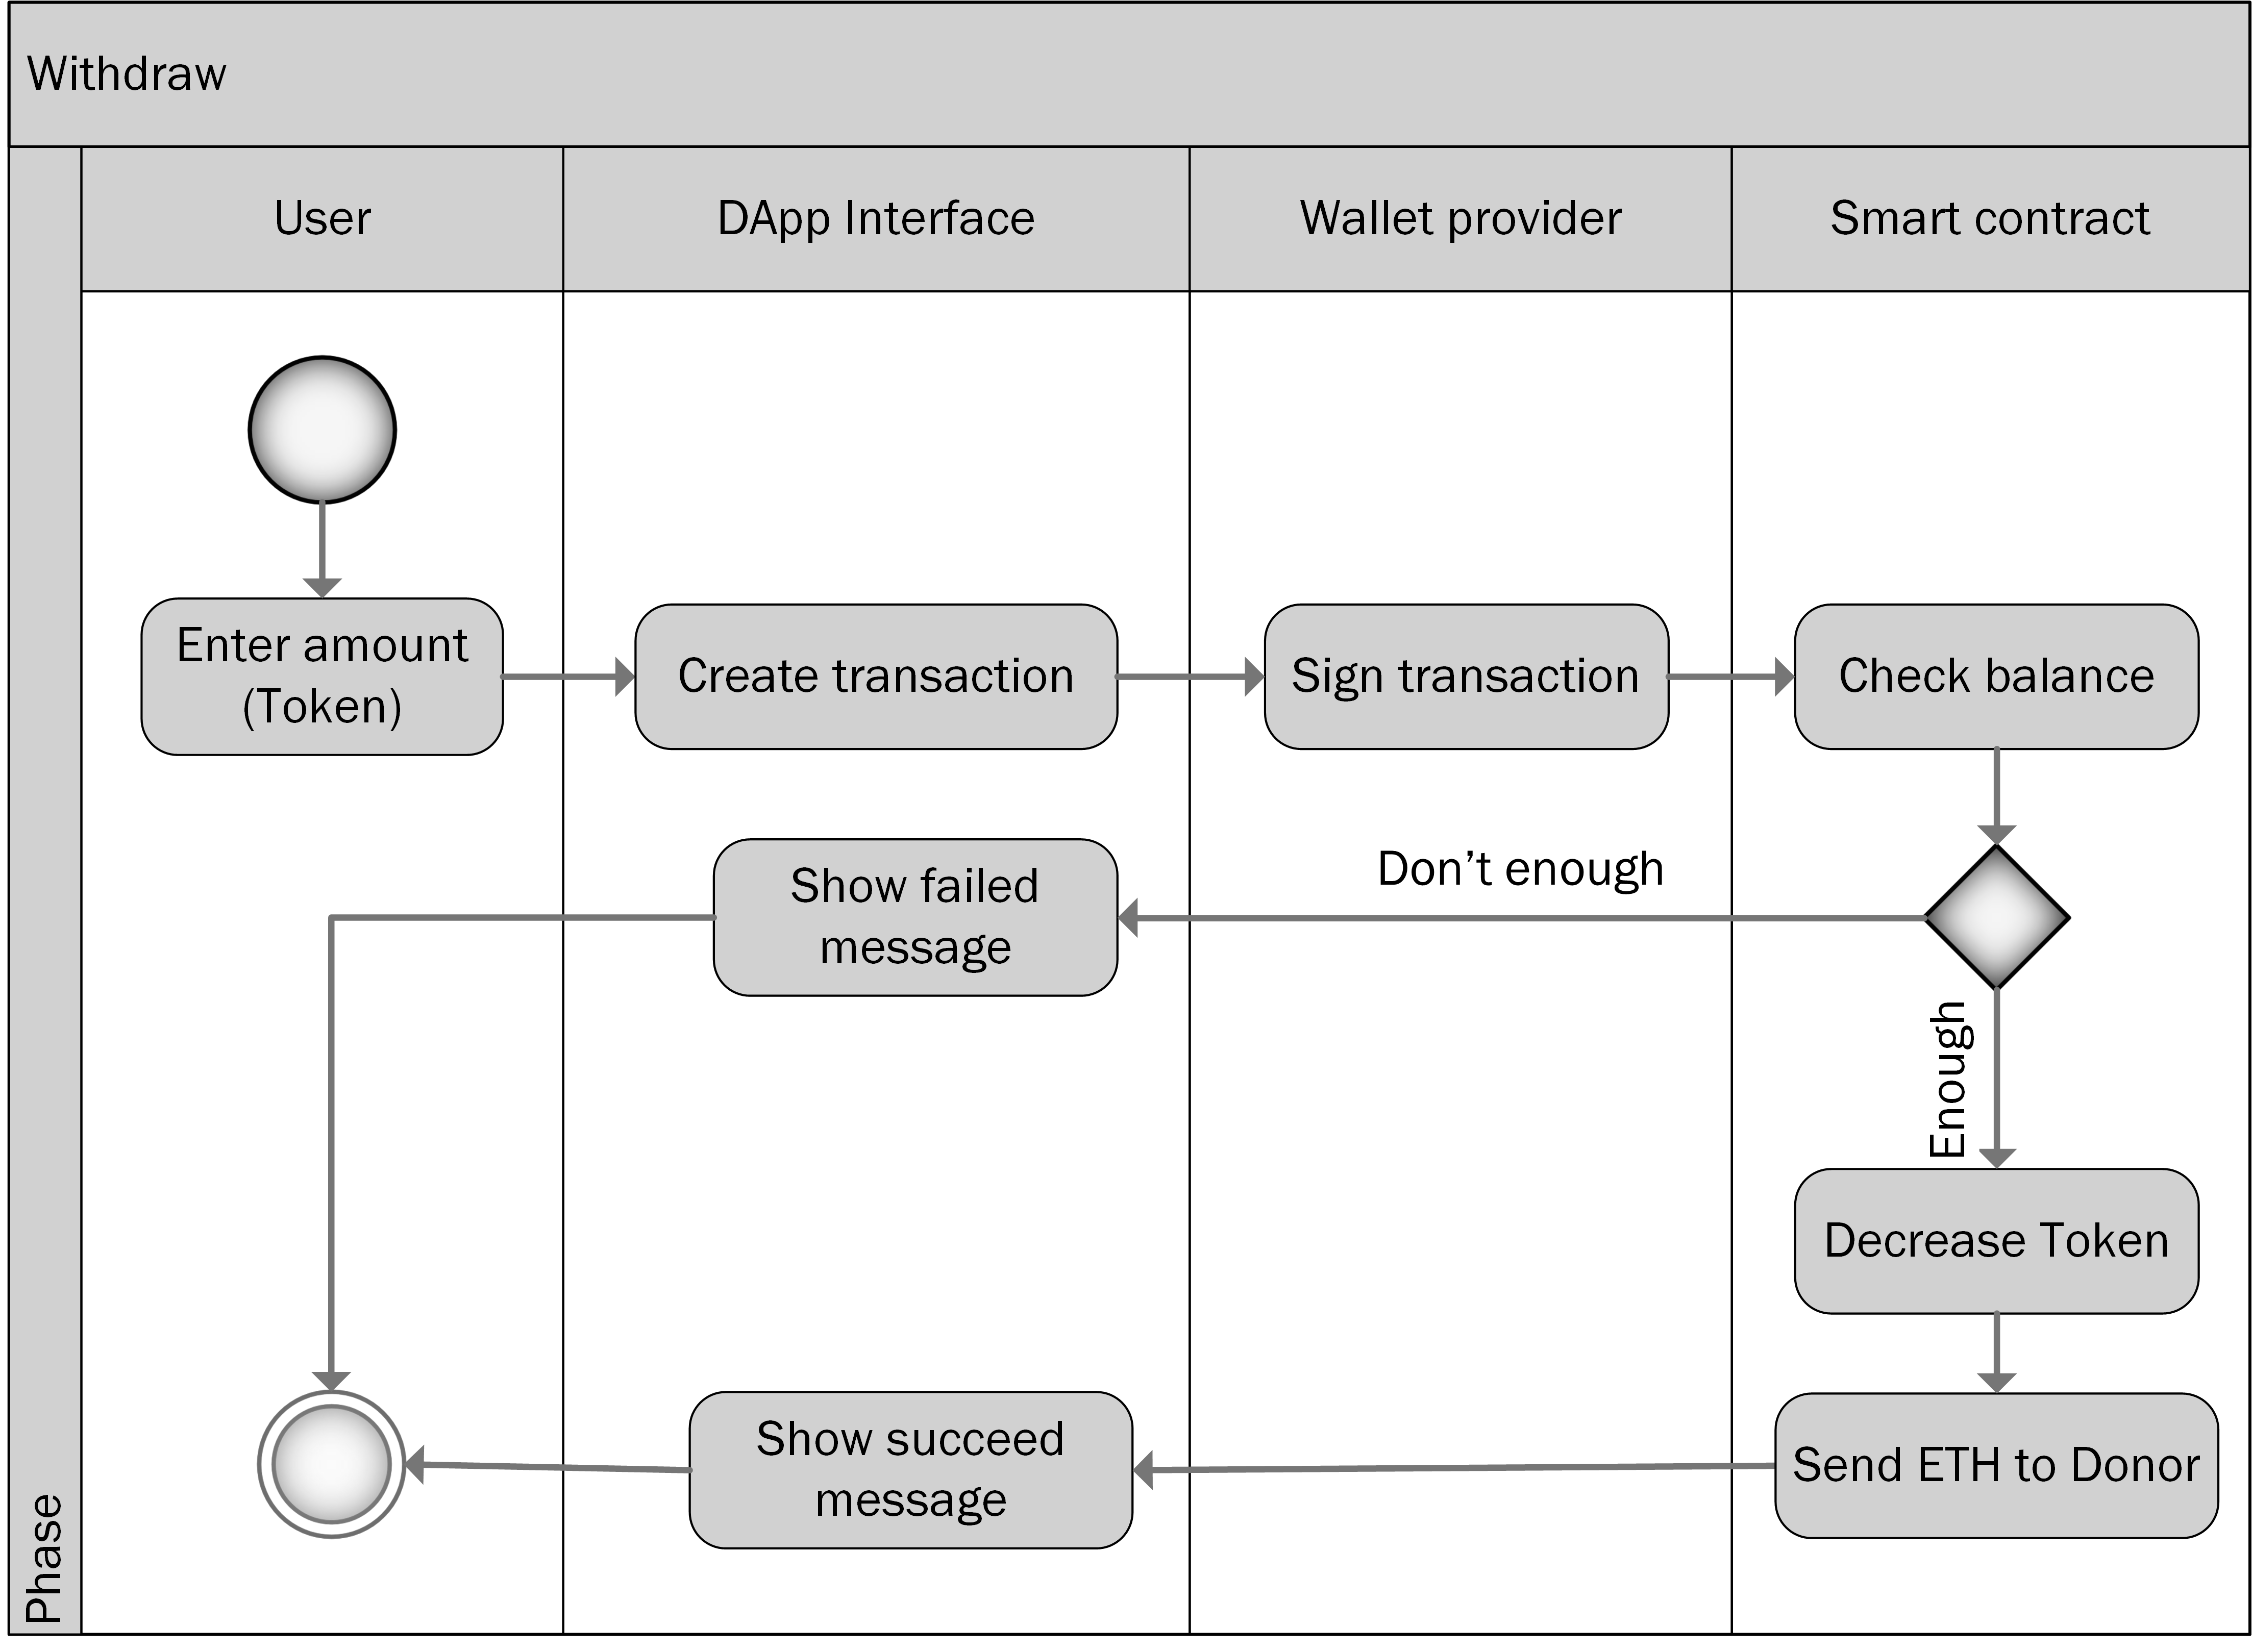
\includegraphics[scale=0.8]{withdraw-activity}
\caption{Sơ đồ hoạt động chức năng rút tiền}
\end{center}
\end{figure}

Tiến trình của hoạt động rút tiền được diễn ra như sau:

\begin{enumerate}[label=(\arabic*)]
\item Người dùng nhập vào lượng token muốn rút.
\item DApp tiến hành tạo \gls{transaction} và gửi đến Wallet provider.
\item Wallet provider tiến hành kí transaction và gửi tới một nút trong mạng blockchain.
\item Một nút trong blockchain nhận được transaction từ Wallet provider, lúc này hàm rút tiền trong hợp đồng thông minh được thực thi. Hợp đồng thông minh tiến hành kiểm tra giá trị token của người dùng. Nếu số dư token đủ thì tiến hành giảm trừ số token tương ứng, sau đó gửi lượng tiền mã hóa \gls{eth} tương ứng cho người dùng, sau đó hiển thị thông báo rút tiền thành công và kết thúc tiến trình. Ngược lại, thông báo lỗi cho người dùng trên giao diện DApp.
\end{enumerate}

\subsection{Chức năng quản lý định danh}
\subsubsection{Mục tiêu}
Do trong \gls{blockchain} mỗi người dùng sẽ được xác định bởi các \gls{address} (địa chỉ), các địa chỉ này hoàn toàn tách biệt với danh tính của người dùng, tức nó không bao gồm danh tính hay bất cứ thông tin nào như địa chỉ IP, định vị, \ldots. Do đó có thể nói mỗi người dùng trên mạng \gls{blockchain} là ẩn danh \cite{henry2018blockchain}. Để tăng tính tin cậy cho chiến dịch gây quỹ thì cần thiết phải gắn mỗi địa chỉ người dùng cho một hồ sơ định danh, vì vậy một địa chỉ người dùng muốn đăng kí tạo chiến dịch thì bắt buộc địa chỉ đó đã có hồ sơ định danh và hồ sơ định danh đó phải được xác minh. Việc tạo lập hồ sơ định danh chỉ bắt buộc với địa chỉ người dùng nào muốn tạo chiến dịch, còn đối với người đóng góp vào chiến dịch thì không bắt buộc.

Hồ sơ định danh có 2 loại thông tin cơ bản là: 

\begin{itemize}
\item \textbf{Thông tin công khai:} là những thông tin cơ bản của người tạo chiến dịch như họ tên, địa chỉ, ngày sinh. Việc công khai thông tin là bắt buộc đối với người tạo chiến dịch.
\item \textbf{Thông tin cá nhân nhạy cảm}: là các thông tin cá nhân bí mật, được dùng để chứng minh cho các thông tin được công khai. Do đó cần lưu trữ thông tin cá nhân nhạy cảm một cách bí mật và toàn vẹn.
\end{itemize}

Yêu cầu về chia sẻ thông tin cá nhân giữa người dùng và người xác minh phải đảm bảo được các yếu tố:

\begin{enumerate}
\item Chỉ có người dùng và người xác minh mới có thể đọc được thông tin.
\item Việc xác minh cho một hồ sơ được minh bạch. Tức biết ai là người đã xác minh cho hồ sơ, và vào thời gian nào.
\end{enumerate}

\subsubsection{Cách hoạt động}
Nhóm tác giả chia làm 2 tiến trình hoạt động cho chức năng này:

\begin{itemize}
\item Tạo lập và lưu trữ hồ sơ định danh.
\item Chia sẻ thông tin hồ sơ định danh.
\end{itemize}

Các đối tượng trong chức năng định danh bao gồm:

\begin{itemize}
\item \textbf{Người tạo lập hồ sơ (người dùng - user):} là người tạo hồ sơ định danh, hay người tạo chiến dịch gây quỹ.
\item \textbf{Người xác minh hồ sơ (verifier)}: người xác minh cho một hồ sơ định danh. Có thể là nhân viên trong hệ thống, tình nguyện viên.
\item \textbf{Người vận hành hệ thống (deployer):} người quản lí danh sách các verifier. Hay người sẽ triển khai hợp đồng thông minh lên \gls{blockchain}.
\end{itemize}

Cách thức tạo lập và lưu trữ hồ sơ định danh được thể hiện ở hình \ref{fig:identity-process-1}. Cụ thể:

\begin{itemize}
\item Người tạo lập hồ sơ định danh tiến hành nhập thông tin định danh.
\item Người tạo lập hồ sơ nhập một chìa khóa bảo vệ hồ sơ định danh, được gọi là \textbf{SecretKey}. SecretKey được dùng cho 2 mục đích:
\begin{enumerate}[label=(\roman*)]
\item Làm khóa (key) cho thuật toán AES dùng để mã hóa các thông tin nhạy cảm của người dùng trước khi lưu trữ.
\item SecretKey sẽ được mã hóa bằng thuật toán RSA bởi khóa công khai của verifier, sau đó chuỗi mã hóa sẽ được lưu trữ trên \gls{blockchain}.
\end{enumerate}
\item Người tạo lập chọn khóa công khai của verifier (chọn một verifier trong danh sách các verifier), khóa này được dùng để mã hóa SecretKey của người tạo lập hồ sơ.
\item Thông tin công khai và khóa bí mật đã mã hóa sẽ được lưu trữ trên hợp đồng thông minh trong blockchain. Thông tin bí mật đã mã hóa sẽ được lưu trữ trên một mạng lưu trữ phi tập trung (ở đây nhóm tác giả đề xuất \acrshort{ipfs}).
\end{itemize}

\begin{figure}[ht!]
\begin{center}
\label{fig:identity-process-1}
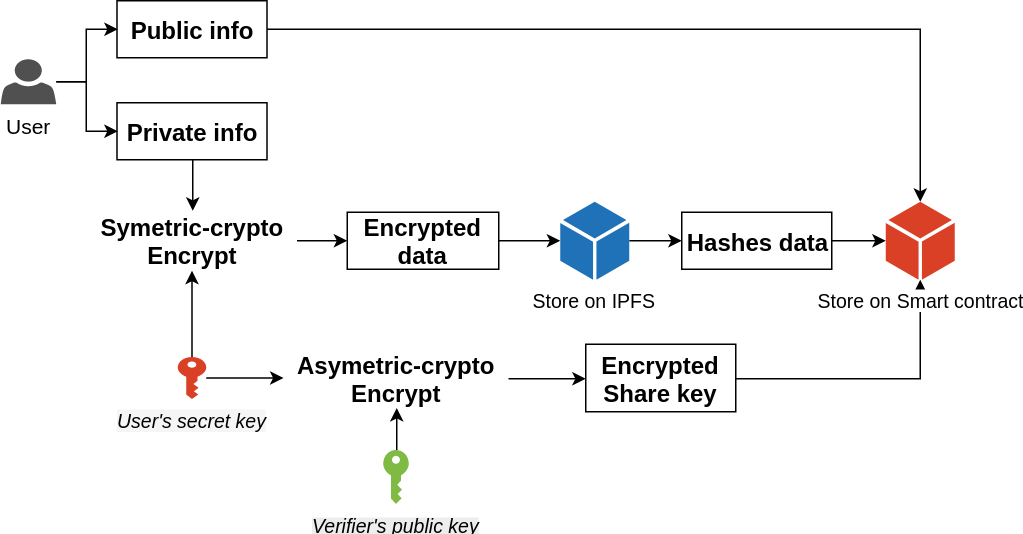
\includegraphics[scale=0.4]{identity-process-1}
\caption{Sơ đồ cách thức lưu trữ hồ sơ định danh}
\end{center}
\end{figure}

Việc chia sẻ hồ sơ định danh là quá trình chia sẻ các thông tin bí mật giữa verifier và người tạo lập hồ sơ phục vụ cho qui trình xác minh hồ sơ. Cách thức chia sẻ hồ sơ định danh được thể hiện trong hình \ref{fig:identity-process-2}:

\begin{itemize}
\item Verifier chọn một hồ sơ định danh của người dùng. Danh sách hồ sơ mà verifier duyệt là các hồ sơ mà người tạo hồ sơ đã chọn khóa công khai tương ứng với verifier đó.
\item Verifier sẽ nhập khóa bí mật (\textit{private key}) để giải mã \textit{SecretKey} của người dùng đã được mã hoá bởi khóa công khai của verifier trước đó.
\item Sau khi có được \textit{SecretKey} của người dùng, verifier sẽ tiến hành giải mã thông tin hồ sơ của người dùng.
\item Verifier dựa vào thông tin bí mật đã giải mã và tiến hành xác minh.
\end{itemize}

\begin{figure}[ht!]
\begin{center}
\label{fig:identity-process-2}
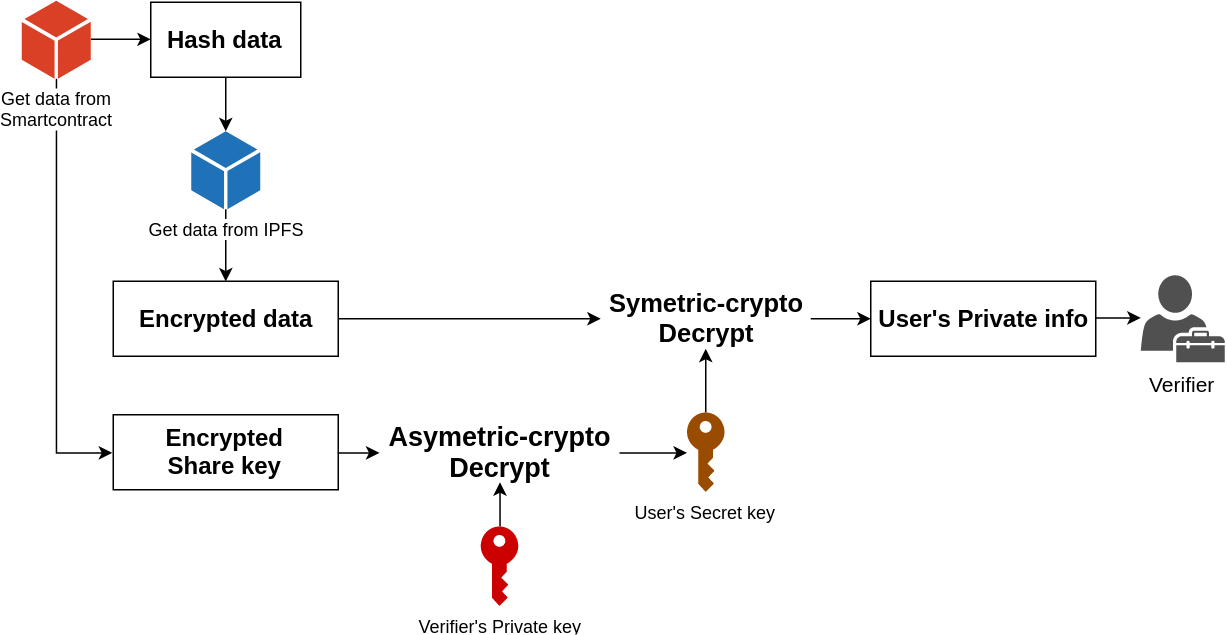
\includegraphics[scale=0.35]{identity-process-2}
\caption{Sơ đồ cách thức chia sẻ thông tin định danh}
\end{center}
\end{figure}

\subsection{Tạo lập và lưu trữ chiến dịch gây quỹ}
\subsubsection{Mục tiêu}
Mục tiêu đối với chức năng tạo lập chiến dịch:

\begin{itemize}
\item Tạo điều kiện tốt nhất và thuận lợi cho người tạo chiến dịch có thể đăng kí được chiến dịch gây quỹ.
\item Người tạo lập chiến dịch cần đăng kí hồ sơ định danh trước khi gọi lệnh đăng kí chiến dịch gây quỹ.
\end{itemize}

Đối với việc lưu trữ chiến dịch gây quỹ:

\begin{itemize}
\item Các thông tin liên quan tài chính thì đặt ưu tiên lưu trữ trên \gls{blockchain}, đảm bảo tính toàn vẹn, công khai và minh bạch.
\item Các dữ liệu không tài chính thì có thể lưu trữ trên cơ sở dữ liệu tập trung, ưu tiên tốc độ đọc dữ liệu.
\end{itemize}
\subsubsection{Cách thức hoạt động}
Sơ đồ hoạt động của tiến trình tạo chiến dịch được thể hiện ở hình \ref{fig:create-campaign-activity}. Tiến trình cụ thể như sau:

\begin{itemize}
\item Đầu tiên người tạo chiến dịch (creator) sẽ tiến hành nhập vào các thông tin của chiến dịch trên DApp Interface. Các thông tin này bao gồm: 
\begin{itemize}
\item Tên chiến dịch gây quỹ.
\item Mô tả ngắn gọn về chiến dịch gây quỹ.
\item Mô tả đầy đủ về chiến dịch.
\item Ảnh (video) về chiến dịch.
\item Mục tiêu gây quỹ.
\item Thời gian gây quỹ.
\item Hồ sơ giải ngân: số giai đoạn giải ngân, số tiền cho từng giai đoạn, phương thức giải ngân.
\end{itemize}
\item DApp Interface tiến hành kiểm tra thông tin mà người tạo đã nhập, nếu thông tin hợp lệ, dữ liệu được xử lí ở tiến trình tiếp theo. Ngược lại, người tạo phải nhập lại thông tin.
\item Dữ liệu sau khi được kiểm tra ở DApp, sẽ được tính toán mã băm (hash) và tính toán một giá trị gọi là \textbf{RefID}, giá trị này được định nghĩa như sau:
\begin{lstlisting} 
RefID = hash(Campaign's name + NOW() + RANDOMIZE())
\end{lstlisting}

Trong đó: \textit{NOW()} là thời gian hiện dưới dạng số (timestamp); \textit{RANDOMIZE()} là một số ngẫu nhiên.
\item RefID cùng với các thông tin chiến dịch như: tên chiến dịch, mô tả ngắn gọn về chiến dịch, mô tả đầy đủ về chiến dịch, ảnh (video) về chiến dịch. Sẽ được gửi tới một cơ sở dữ liệu tập trung của hệ thống (Centralized database). Lúc này cơ sở dữ liệu tập trung này sẽ kiểm tra lại dữ liệu được gửi tới lần nữa, nếu dữ liệu hợp lệ sẽ tiến hành lưu xuống cơ sở dữ liệu. Ngược lại, dữ liệu không hợp lệ sẽ bắt người tạo phải nhập lại thông tin.
\item Khi dữ liệu về mô tả chiến dịch được lưu ở cơ sở dữ liệu tập trung thành công thì DApp sẽ tiến hành tạo giao dịch có kèm mã băm đã tính toán trước đó cùng các thông tin như: mục tiêu gây quỹ, thời gian gây quỹ, hồ sơ giải ngân, RefID. Sau đó transaction được gửi tới Wallet Provider.
\item Wallet Provider tiến hành kí cho \gls{transaction} bằng khóa bí mật của người tạo. Sau đó \gls{transaction} được gửi tới một nút trong mạng blockchain, để hợp đồng thông minh xử lí.
\item Khi giao dịch được gửi tới, hợp đồng thông minh sẽ kiểm tra lại lần nữa các đầu vào, nếu dữ liệu hợp lệ thì dữ liệu được lưu. Ngược lại trả về thông báo lỗi cho người dùng.
\end{itemize}

\begin{figure}[ht!]
\begin{center}
\label{fig:create-campaign-activity}
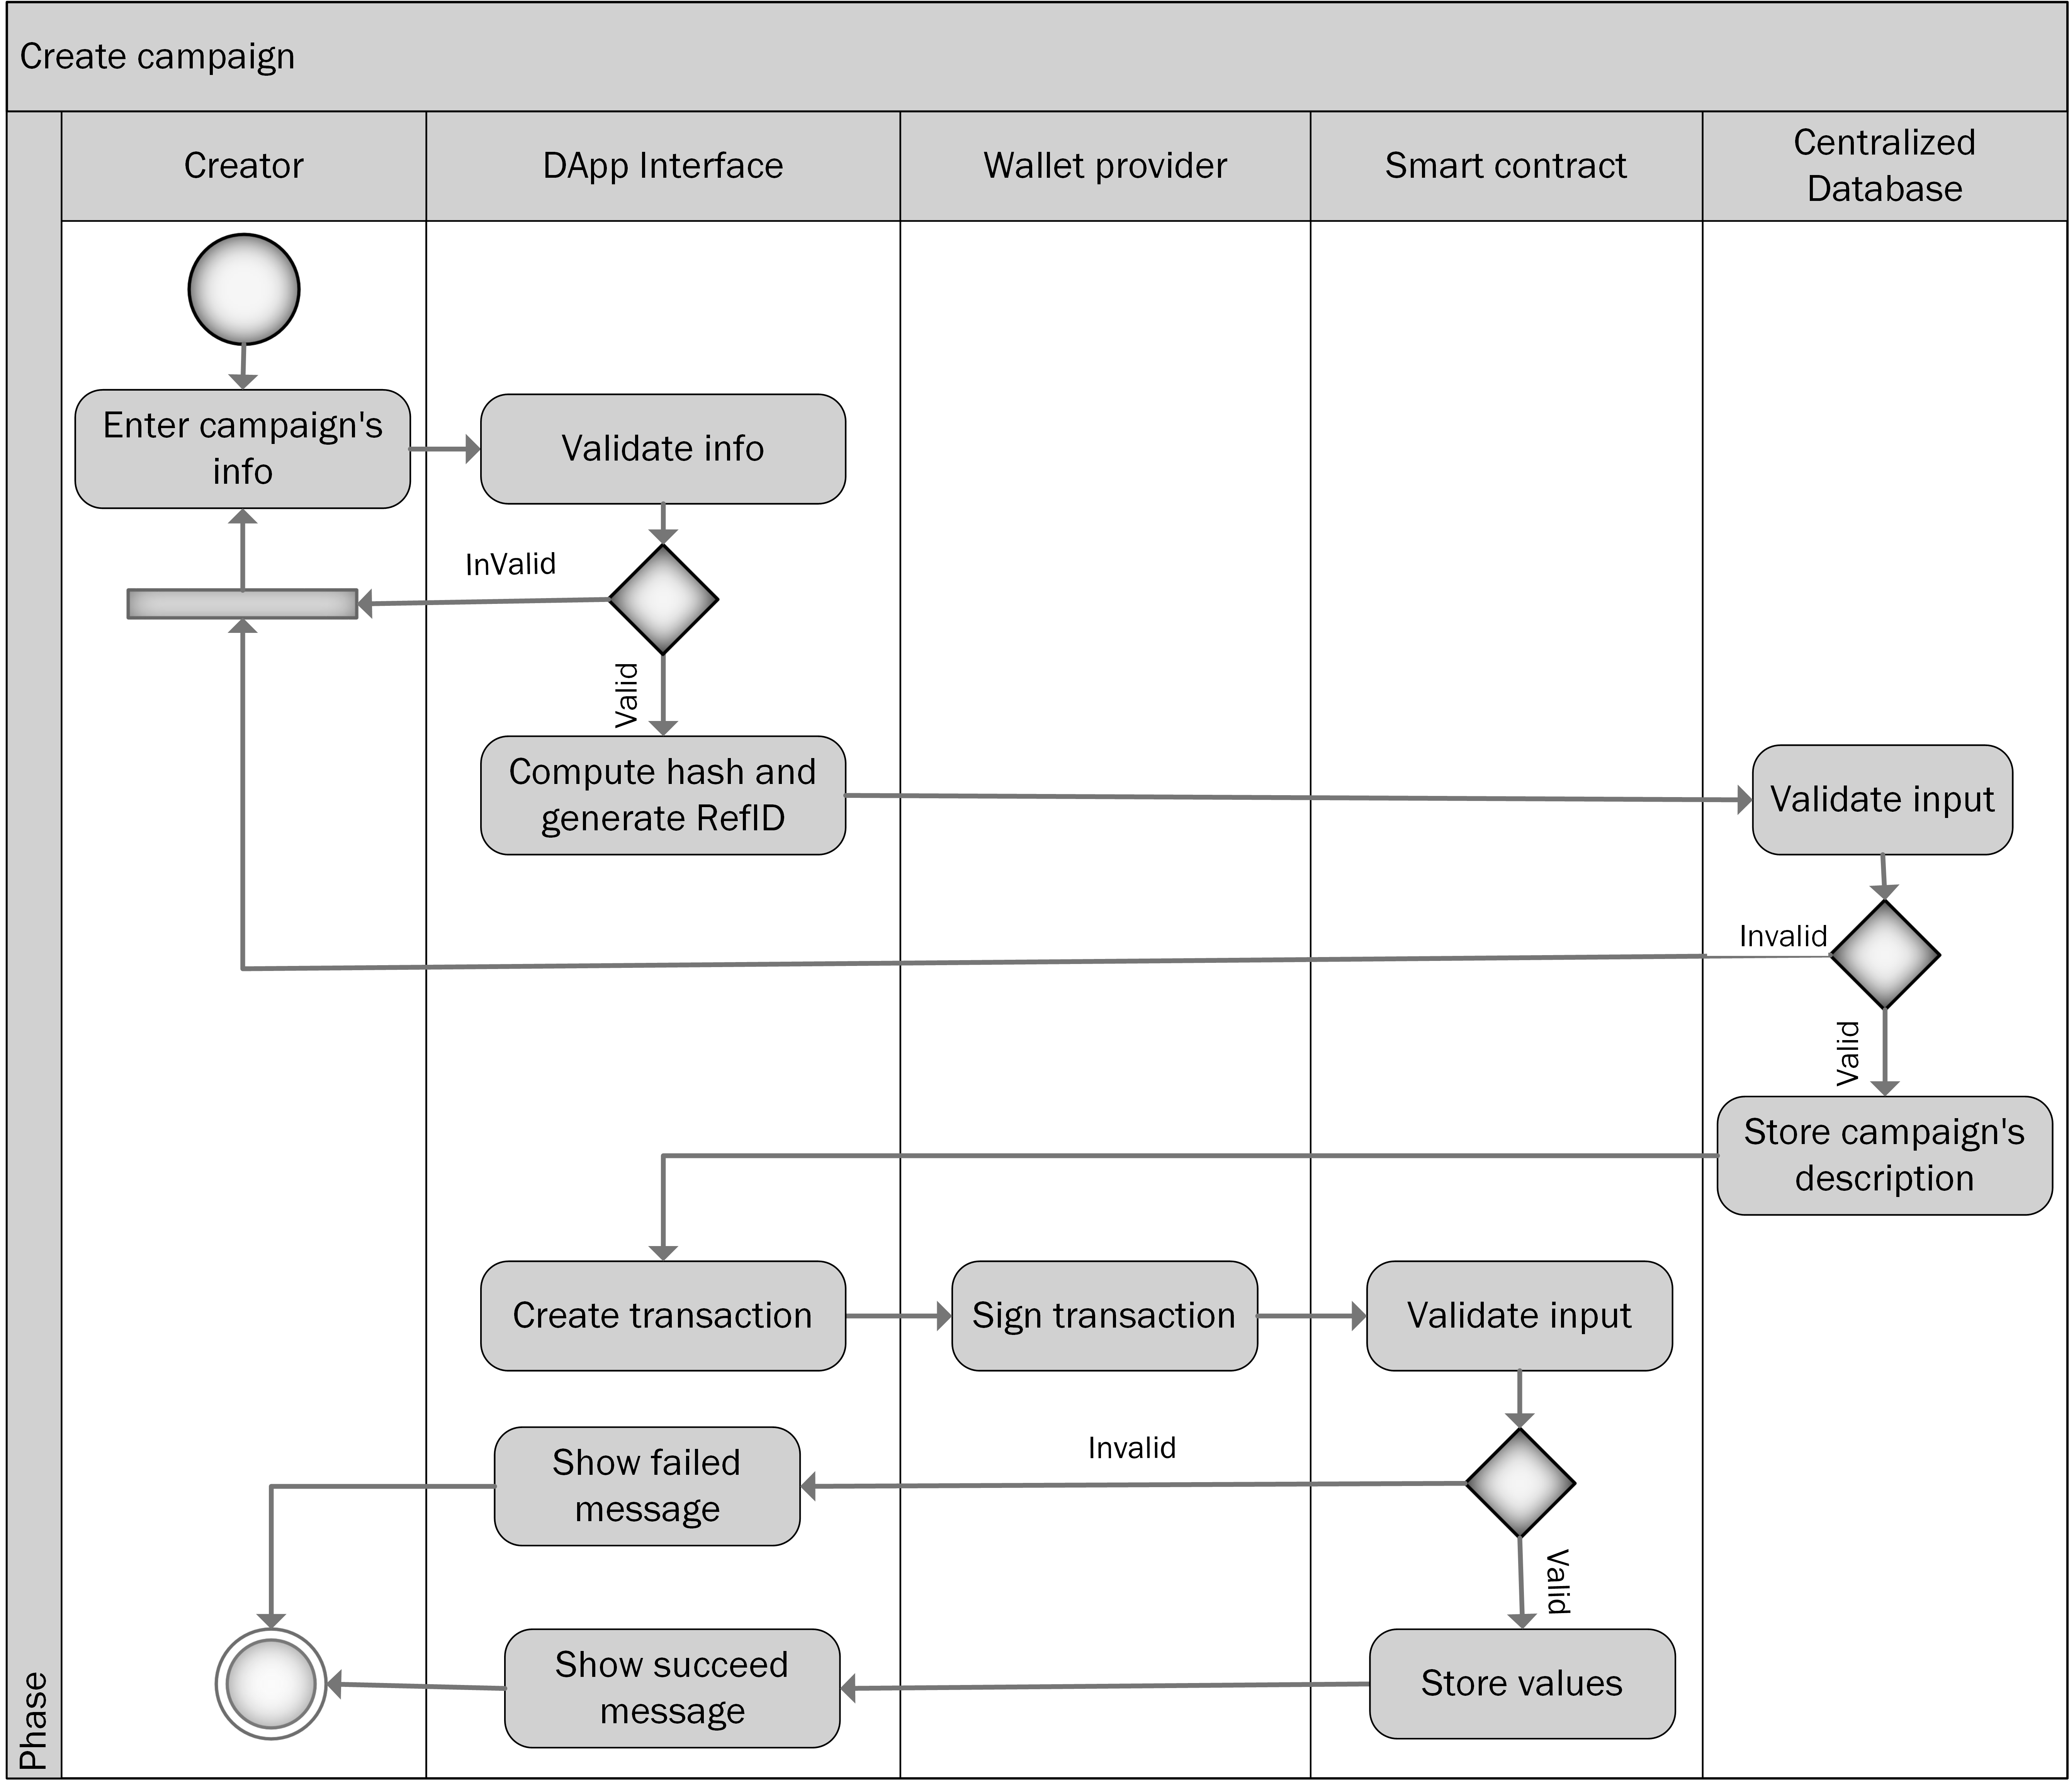
\includegraphics[scale=0.65]{create-campaign-activity}
\caption{Sơ đồ hoạt động tiến trình tạo lập chiến dịch}
\end{center}
\end{figure}

\subsection{Chức năng giải ngân}
\subsubsection{Mục tiêu}
Việc giải ngân được thực hiện khi chiến dịch gây quỹ đạt được mục tiêu gây quỹ. Và giải ngân đối với chiến dịch sẽ được phân làm hai loại:

\begin{itemize}
\item \textbf{Giải ngân một giai đoạn} - sau khi chiến dịch gây quỹ hoàn thành mục tiêu gây quỹ trong thời gian đặt ra, thì người tạo chiến dịch có thể gọi lệnh giải ngân và rút được tiền từ chiến dịch.
\item \textbf{Giải ngân theo nhiều giai đoạn} - với một số chiến dịch có thể thực hiện theo nhiều giai đoạn khác nhau, thì việc giải ngân theo nhiều giai đoạn nhằm mục tiêu:
\begin{itemize}
\item Buộc người tạo chiến dịch có trách nhiệm báo cáo tiến độ thực hiện chiến dịch.
\item Tăng cường quyền của người đóng góp bằng cách bỏ phiếu đồng ý xác nhận giải ngân cho chiến dịch theo từng giai đoạn.
\end{itemize}
\end{itemize}

\subsubsection{Cách thức hoạt động}
Chức năng giải ngân bao gồm các tiến trình:

\begin{itemize}
\item Tạo hồ sơ giải ngân.
\item Bỏ phiếu đồng ý giải ngân.
\item Gọi lệnh giải ngân.
\end{itemize}

\paragraph{Tiến trình tạo hồ sơ giải ngân:} hồ sơ giải ngân sẽ được người tạo chiến dịch nhập vào lúc đăng kí chiến dịch gây quỹ, các thông tin trong hồ sơ giải ngân bao gồm:

\begin{itemize}
\item Số giai đoạn thực hiện giải ngân. Nếu giai đoạn giải ngân là $ 1 $ thì các thông tin bên dưới có thể bỏ trống.
\item Số tiền cần cho mỗi giai đoạn (tổng tiền ở các giai đoạn sẽ bằng mục tiêu gây quỹ).
\item Tùy chọn chế độ giải ngân, có $ 4 $ chế độ:
\begin{itemize}
\item \textbf{Flexible} -- đủ điều kiện giải ngân ở giai đoạn nào thì được rút tiền ở giai đoạn đó.
\item \textbf{Fixed} -- muốn rút tiền ở giai đoạn tiếp theo thì giai đoạn trước đó phải đủ điều kiện giải ngân.
\item \textbf{TimingFlexible} -- người tạo chiến dịch sẽ ấn định thời gian thực hiện cho mỗi giai đoạn, khi hết thời gian ấn định của giai đoạn hiện tại thì mới có thể thực hiện lệnh bỏ phiếu giải ngân và rút tiền cho giai đoạn tiếp theo. 
\item \textbf{TimingFixed} -- người tạo chiến dịch sẽ ấn định thời gian thực hiện cho mỗi giai đoạn, khi hết thời gian ấn định của giai đoạn hiện tại thì mới có thể thực hiện lệnh bỏ phiếu giải ngân và rút tiền cho giai đoạn tiếp theo. Nếu giai đoạn hiện tại không đủ điều kiện giải ngân thì giai đoạn sau sẽ không được rút tiền.
\end{itemize}
\end{itemize}

\paragraph{Tiền trình bỏ phiếu giải ngân cho mỗi giai đoạn} -- tiến trình bỏ phiếu được đặc tả như sau:

\begin{itemize}
\item Chỉ có người đã đóng góp tiền cho chiến dịch thì mới có quyền bỏ phiếu cho chiến dịch đó.
\item Việc bỏ phiếu đồng ý giải ngân được thực hiện cho từng giai đoạn giải ngân của chiến dịch, không bỏ phiếu cho toàn bộ chiến dịch.
\item Với mỗi lá phiếu sẽ có hai tùy chọn: Đồng ý hoặc Không đồng ý giải ngân.
\item Số phiếu ``Đồng ý'' đạt từ 50\% trên tổng số người đã đóng góp vào chiến dịch và tổng số tiền mà những những người đồng ý giải ngân phải đạt tỉ lệ trên 50\% tổng số tiền mục tiêu gây quỹ thì được xem là đủ điều kiện giải ngân.
\end{itemize}

\paragraph{Tiến trình gọi lệnh giải ngân} -- việc gọi lệnh giải ngân sẽ có hai trường hợp:

\begin{itemize}
\item Đối với chiến dịch chỉ có một giai đoạn giải ngân: được rút toàn bộ số tiền gây quỹ được nếu hoàn thành mục tiêu gây quỹ trong thời gian đặt ra.
\item Chiến dịch từ 2 giai đoạn thực hiện trở lên: giai đoạn đầu tiên sẽ được rút tiền mà không cần người đóng góp bỏ phiếu. Từ giai đoạn thứ hai trở đi, cần đạt điều kiện về bỏ phiếu giải ngân thì mới được rút tiền.
\end{itemize}

\subsection{Hoàn tiền chiến dịch gây quỹ}
\subsubsection{Mục tiêu}
Chức năng này giúp người đóng góp tiền vào chiến dịch có thể thực hiện hoàn tiền trong hai trường hợp:

\begin{itemize}
\item Trường hợp 1: hoàn tiền khi đang trong thời gian gây quỹ. Việc hoàn tiền này được thực hiện theo yêu cầu của người đóng góp.
\item Trường hợp 2: hoàn tiền sau khi hết thời gian gây quỹ. Điều kiện để hoàn tiền trong trường hợp này là chiến dịch không đạt được mục tiêu gây quỹ trong thời gian đặt ra. Việc hoàn tiền này phải diễn ra một cách tự động. Tức người đóng góp không cần thực hiện bất kì thao tác gì.
\end{itemize}

\subsubsection{Cách hoạt động}
Phần này, nhóm tác giả tập trung vào việc hoàn tiền tự động khi chiến dịch kêu gọi quỹ thất bại (không đạt được mục tiêu kêu gọi quỹ).

Có hai giải pháp thiết kế thuật toán đáp ứng yêu cầu đặt ra:

\begin{itemize}
\item \textbf{Giải pháp 1 -- chủ động:} thực hiện chạy chủ động lặp đi lặp lại một hàm nào đó trong hợp đồng thông minh để kiểm tra chiến dịch đã kết thúc và cập nhật các giá trị sau khi hết thời gian gây quỹ.
\item \textbf{Giải pháp 2 -- bị động:} không thực hiện bất kì thay đổi nào về giá trị token của người dùng được lưu trữ trong hợp đồng thông minh khi chiến dịch thất bại. Khi người dùng kiểm tra số dư hoặc thực hiện rút tiền sẽ tiến hành kiểm tra số dự thực tế dựa vào trạng thái thành công hay thất bại của các chiến dịch gây quỹ.
\end{itemize}

Với hai giải pháp được nêu trên, nhóm tác giả chọn giải pháp thứ 2 để thiết kế, với lí do sau:

\begin{itemize}
\item Chi phí của giải pháp thứ hai thấp hơn đáng kể so với giải pháp thứ nhất. Do việc kiểm tra số dư chỉ đơn thuần là đọc dữ liệu.
\item Đặc điểm của \gls{blockchain} là để thay đổi các giá trị đã lưu trữ thì cần tạo ra các transaction gọi đến các hàm trong hợp đồng thông minh thì hàm đó mới được khởi chạy và thay đổi dữ liệu. Do đó hiện tại, Ethereum chưa hỗ trợ việc lập lịch cho một giao dịch tự động chạy theo thời gian định trước. Vì vậy để hiện thực giải pháp 1 cần chạy một máy chủ thực hiện việc gửi transaction theo lịch định sẵn. Việc tạo một máy chủ ở đây có thể là một điểm chết. Và với mỗi giao dịch được chạy tự động như vậy về lâu dài sẽ tốn một chi phí không nhỏ cho người vận hành.
\end{itemize}

Với giải pháp thứ hai được chọn, nhóm tác giả đề xuất công thức tính toán cho số dư token của người dùng trong hệ thống như sau:

%\fbox{$ T = T_0 - T_{donated} $}

\noindent\fbox{\begin{minipage}{\dimexpr\textwidth-2\fboxsep-2\fboxrule\relax}
\centering
$ T = T_0 - T_{donated} $
\end{minipage}}

Trong đó:

\begin{itemize}
\item $T$ là số dư thực tế của người dùng.
\item $T_0$ là số dư ban đầu người dùng gửi vào hợp đồng thông minh.
\item $T_{donated}$ là số token mà người dùng đã đóng góp vào chiến dịch. Các chiến dịch ở đây bao gồm các chiến dịch đang kêu gọi gây quỹ và chiến dịch đã kêu gọi thành công. Không bao gồm chiến dịch kêu gọi thất bại.
\end{itemize}

\section{Tổ chức dữ liệu}
\subsection{Dữ liệu phi tập trung}
Cấu trúc hợp đồng thông minh được thể hiện ở hình \ref{fig:smartcontract-structure}. Cụ thể trong hệ thống có các hợp đồng thông minh sau:

\begin{itemize}
\item \textbf{Wallet} -- đây là hợp đồng chứa mã lưu trữ và xử lí các tác vụ liên quan đến tài chính trong hệ thống, bao gồm các tác vụ như nộp tiền và rút tiền trong hệ thống.
\item \textbf{Campaigns} -- là một contract chứa nhiều mã xử lí nhất trong hệ thống, bao gồm việc lưu trữ thông tin liên quan đến chiến dịch, các tác vụ như tạo chiến dịch, đóng góp tiền vào một chiến dịch, giải ngân.
\item \textbf{Identity} -- chứa mã lưu trữ và xử lí các tác vụ liên quan đến thông tin định danh. Các tác vụ trên contract này như: đăng kí hồ sơ định danh, duyệt hồ sơ định danh.
\item \textbf{Disbursement} -- chứa mã lưu trữ thông tin giải ngân của chiến, tác vụ bỏ phiếu giải ngân được contract này xử lí. 
\end{itemize}

\begin{figure}[ht!]
\begin{center}
\label{fig:smartcontract-structure}
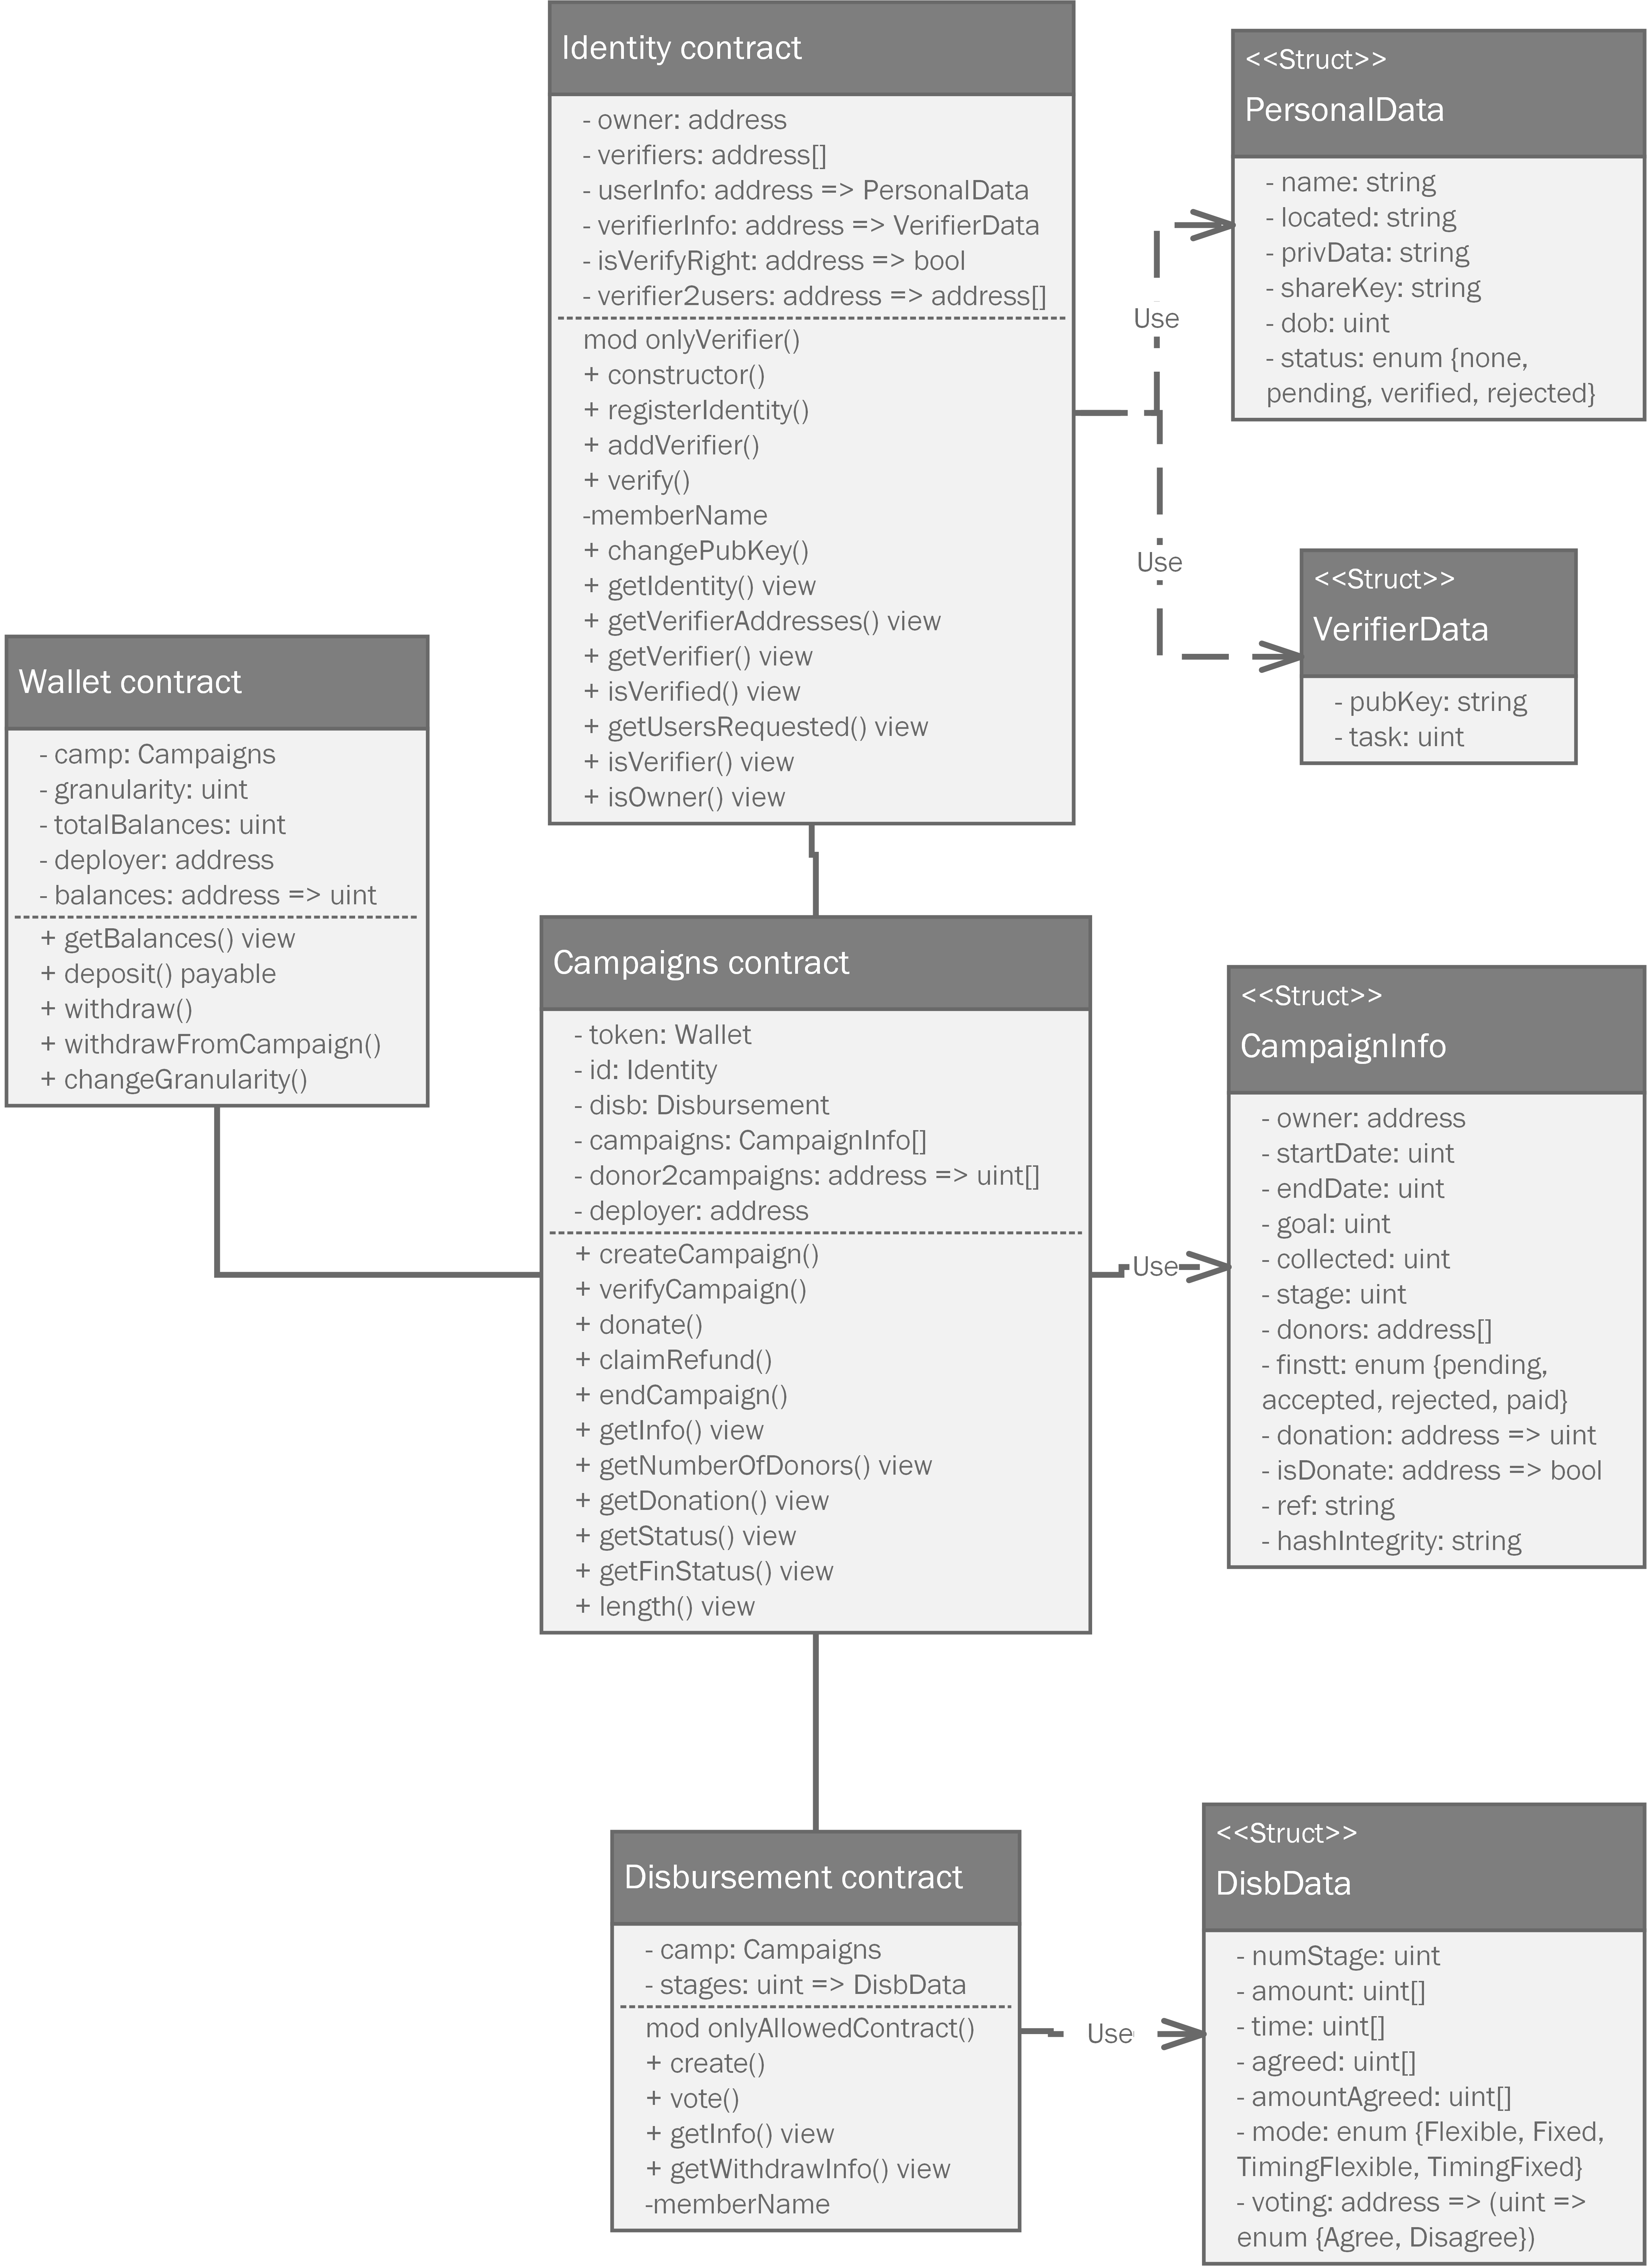
\includegraphics[scale=0.65]{smartcontract-structure}
\caption{Kiến trúc hợp đồng thông minh}
\end{center}
\end{figure}

\subsection{Dữ liệu tập trung}
Các dữ liệu được lưu tại cơ sở dữ liệu tập trung bao gồm các thông tin mô tả chiến dịch:

\begin{itemize}
\item Tên chiến dịch.
\item Thông tin ngắn gọn về chiến dịch.
\item Mô tả chi tiết về chiến dịch.
\item Hình ảnh mô tả về chiến dịch dưới dạng đường dẫn.
\end{itemize}

Bảng thiết kế cơ sở dữ liệu được mô tả ở hình \ref{fig:db-design}.

\begin{figure}[ht!]
\begin{center}
\label{fig:db-design}
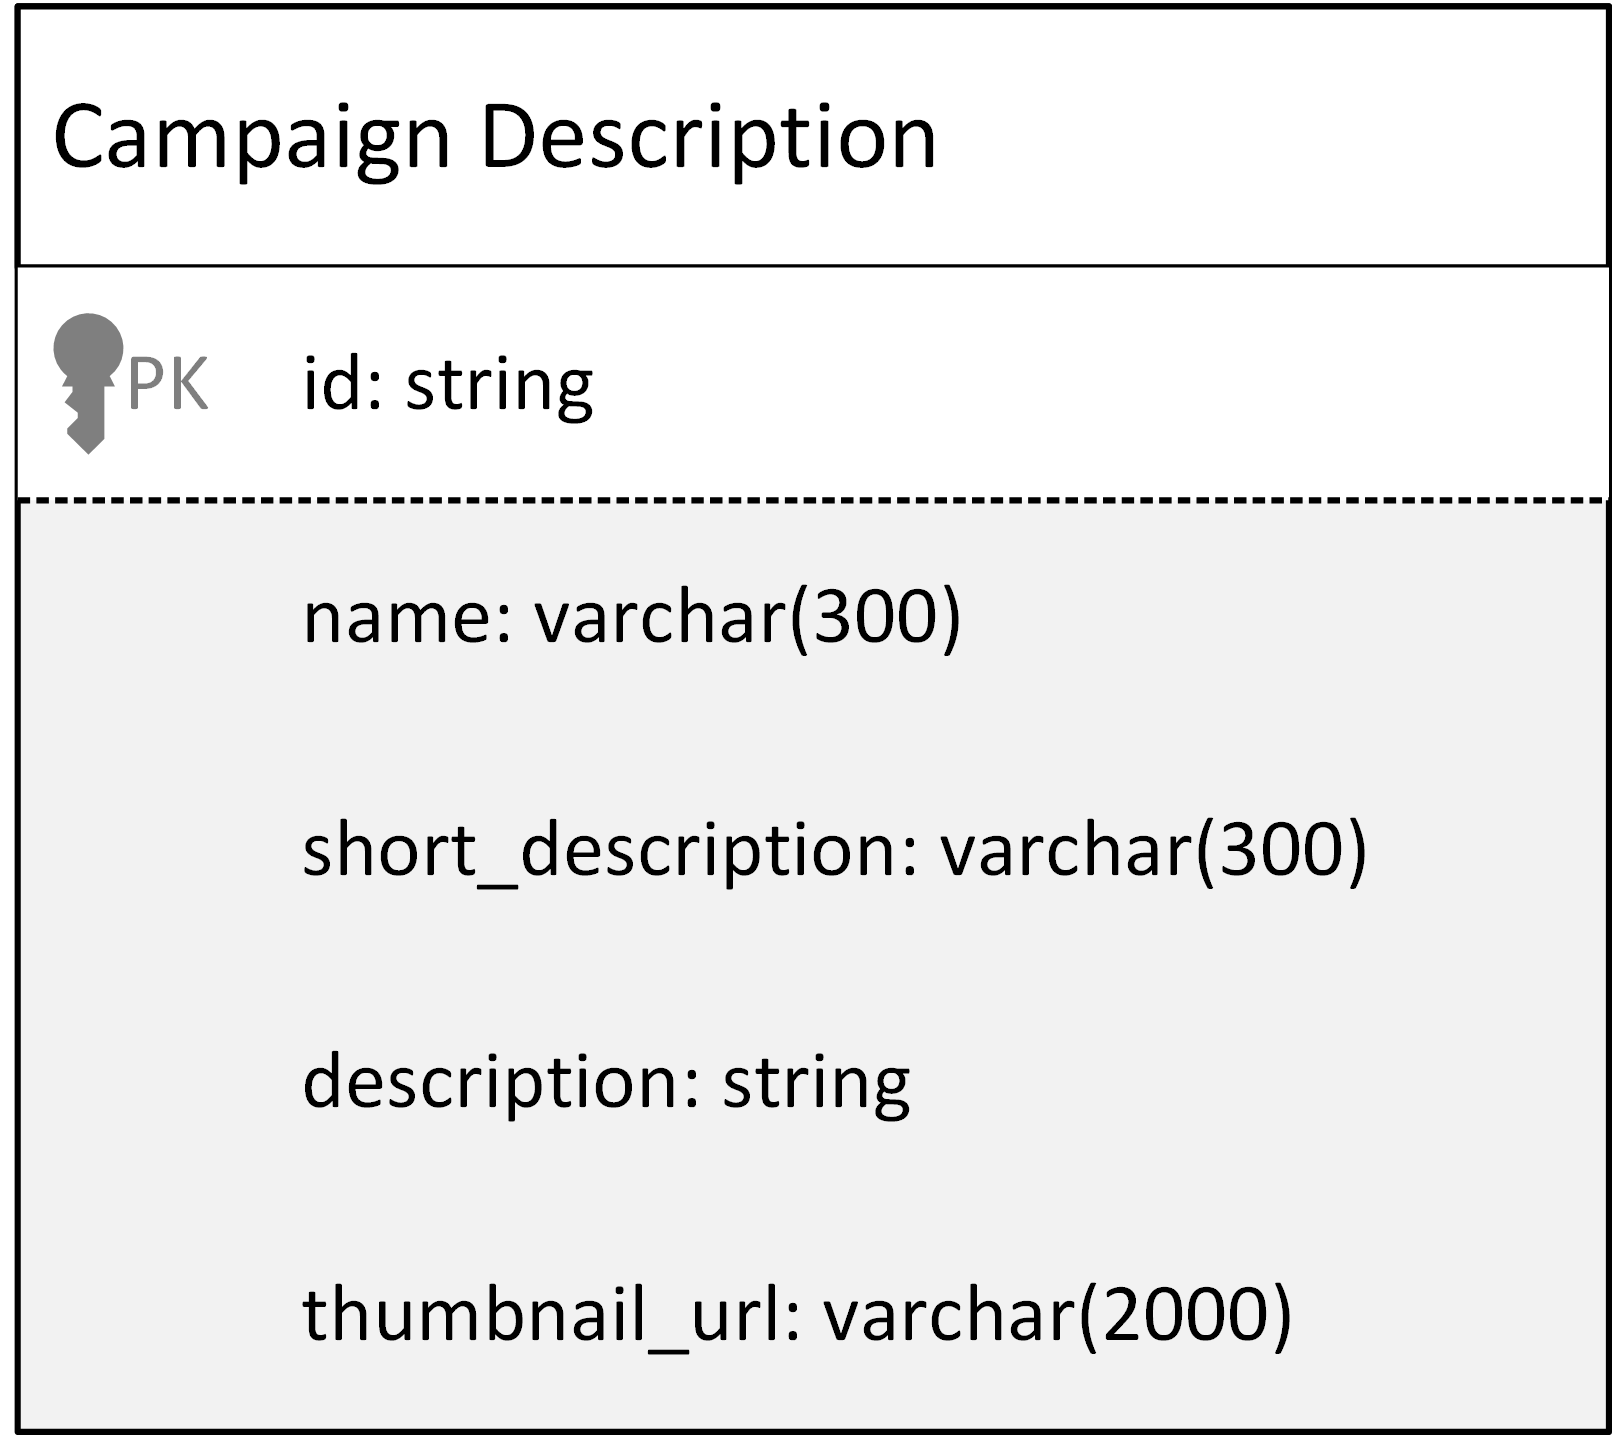
\includegraphics[scale=1]{db-design}
\caption{Thiết kế cơ sở dữ liệu tập trung}
\end{center}
\end{figure}

\end{document}